% introduzione al corso di codifica del testo anno accademico 2018/2019

\documentclass{beamer}
    
%    \usepackage[english]{babel}
    %\usepackage[latin1]{inputenc}
    %\usepackage[T1]{fontenc}

\mode<presentation>{
  \setbeamertemplate{background canvas}[vertical shading]
  \usetheme{Berkeley}
  \useoutertheme{himinfolines}
}
  
\usepackage{ucs}
\usepackage[utf8]{inputenc}
\usepackage[english,polutonikogreek,italian,UKenglish,british]{babel}
\usepackage{graphicx}
\usepackage{colortbl}
\usepackage{multicol}
\usepackage{ulem}
\usepackage{verbatim}
\usepackage{alltt}
\usepackage{ccicons}
\usepackage{MnSymbol,wasysym}
\usepackage{tikzsymbols}
\usepackage{textcomp}
\usepackage{xmpincl}

\usepackage{parskip}
\setcounter{nframes}{90}
\setcounter{nframe}{1}
\setbeamercovered{dynamic}
\newenvironment{grcenv}{\begin{otherlanguage}{greek}}{\end{otherlanguage}}
\newcommand{\g}[1]{\textgreek{#1}}
\definecolor{darkgreen}{rgb}{0,0.5,0}
\definecolor{darkblue}{rgb}{0,0,0.5}
\definecolor{grey}{rgb}{0.5,0.5,0.5}
\setcounter{tocdepth}{5}

\makeatletter

\makeatother
%\includexmp{LicencesAndLicensing}

%frame00 metadata
	\title{Introduzione sistema git per edizioni collaborative}
	\author[A.M. Del Grosso]{Angelo Mario Del Grosso}
	%\institute{DIGITAL TOOLS FOR HUMANISTS SUMMER SCHOOL 2019}
    %\institute{\texttt{angelo.delgrosso@ilc.cnr.it} \\\bigskip\textit{CNR-ILC-LicoLab} \\\bigskip\url{http://licolab.ilc.cnr.it/}}
    \institute{\texttt{angelo.delgrosso@ilc.cnr.it} \\\bigskip\textit{CNR-ILC-LicoLab}}
    \date{Istituto di Linguistica Computazionale ``A. Zampolli'', \today}
    \AtBeginSection[]{
    \begin{frame}<beamer>
    \addtocounter{nframe}{1}
    \footnotesize
    \frametitle{Progress status}
    \tableofcontents[currentsection,hideothersubsections]
    \end{frame}
    }

\begin{document}

\begin{frame}
	\maketitle
\end{frame}

\begin{frame}
	\frametitle{Outline}
	\tableofcontents
\end{frame}

\section{Self Introduction}

\begin{frame}
	\frametitle{What is my work about}
	\addtocounter{nframe}{1}

	\begin{block}{Digital and Computational Philology}
		%slide di presentazione: chi sono, piccola bio, di cosa mi occupo
		%\\prendere dal curriculum alcuni pezzi mettere mail istituzionale ed eventualmente telefono
		Analisi, progettazione e sviluppo di componenti software per sistemi di linguistica e filologia digitale/computazionale volti alla produzione, rappresentazione, trattamento, fruizione e interrogazione di testi di tradizione medievale, a stampa e di autori moderni e contemporanei.
	\end{block}

	% \begin{block}{Modelli Object Oriented per il Textual Scholarship}
	% 	Impiego delle nuove tecnologie nell’ambito delle Digital Humanities (DH) per la progettazione object–oriented di strumenti digitali Web–based rispondenti alle esigenze degli utenti accademici, studenti e sviluppatori.
	% \end{block}


\end{frame}

\begin{frame}
	\frametitle{Topic of the talk}
	\addtocounter{nframe}{1}

	\begin{center}
		
\includegraphics[width=.7\textwidth]{./imgs/git-github.jpeg}
	\end{center}

	%\begin{itemize}
	%	\item<1-> Introduzione
	%	\item<2-> Codifica dei Caratteri
	%   \item<3-> Codifica dei Testi
	%   \item<4-> Ecosistema XML (Linee Guida TEI)
	%   \item<5-> Conclusioni
	%\end{itemize}

\end{frame}


\begin{frame}
	\frametitle{First of all}
	\addtocounter{nframe}{1}

	\begin{itemize}
		\item<1-> Version Control Systems (VCSs) 
		\item<2-> Git usage through the main CLI commands 
		\item<3-> Cloning, modifying, contributing, diffing, logging
		\item<4-> Working with remotes
		\item<5-> GitHub hosting service (little tips on projects and organization)
		\item<6-> Stashing and Branching model (\emph{NO WITHIN THIS TALK})
		\item<7-> Adavanced git tools (\emph{NO WITHIN THIS TALK})
	\end{itemize}

\end{frame}



\begin{frame}
	\frametitle{Topic of the talk}
	\addtocounter{nframe}{1}

	\begin{block}{Book which this workshop is derived from}
		\begin{center}
			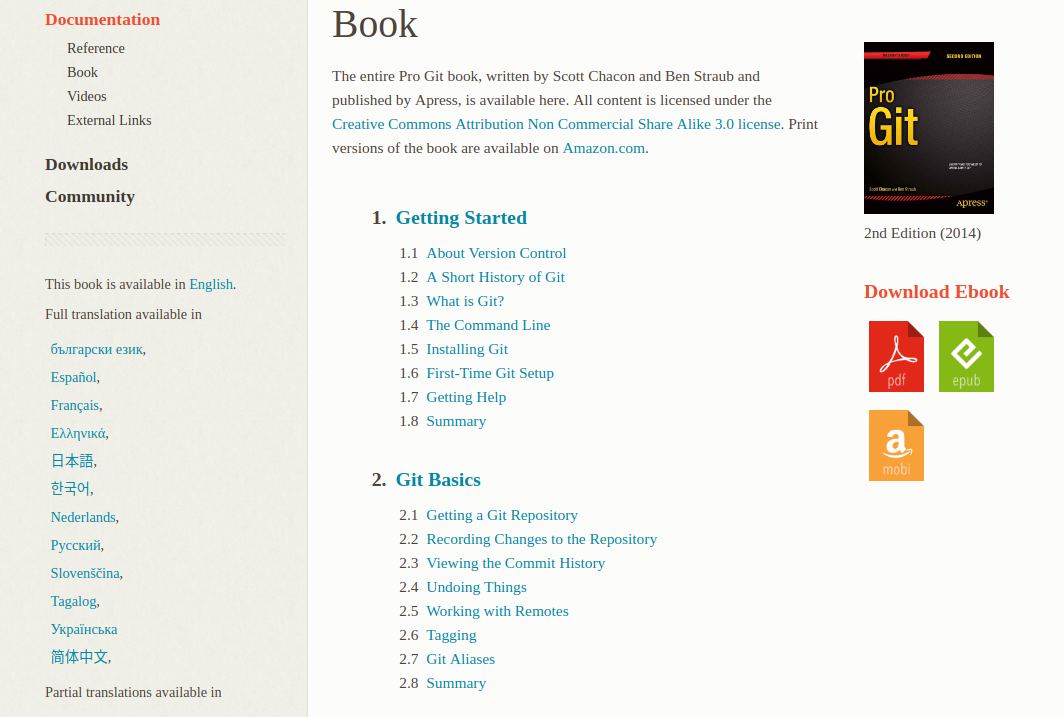
\includegraphics[width=.7\textwidth]{./imgs/GIT-BOOK.png}
		\end{center}
	\end{block}

	\texttt{https://git-scm.com/book/en/v2}
	
\end{frame}

\begin{frame}
	\frametitle{Topic of the workshop}
	\addtocounter{nframe}{1}

	\begin{block}{Working Session - Example of using Git}
		\begin{center}
			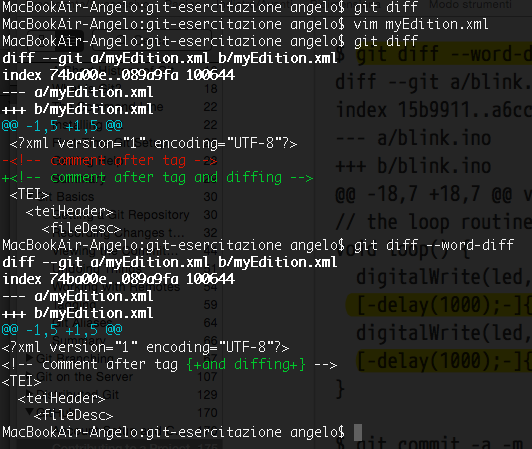
\includegraphics[width=.7\textwidth]{./imgs/Diffing-line-word.png}
		\end{center}
	\end{block}

\end{frame}

\section{VCS Introduction}
% sezione intro frame 
\begin{frame}
    \frametitle{Git and GitHub}
    \framesubtitle{Getting started with Git}
    \addtocounter{nframe}{1}
    
    \begin{block}{--}
    \end{block}

    \begin{block}{--}
    \end{block}

\end{frame}

% sezione intro frame 00
\begin{frame}
    \frametitle{Git intro}
    \framesubtitle{Getting started with Git}
    \addtocounter{nframe}{1}
    
    \begin{block}{VCS}
        Version control (VCS) is a system that records changes to a file or set of files over time so that you can recall specific versions later.
    \end{block}

    \begin{block}{Benefits}
        \begin{itemize}
            \item It allows you to revert selected files back to a previous state
            \item compare changes over time
            \item who last modified something that might be causing a problem
            \item \dots
        \end{itemize}
    \end{block}

\end{frame}


% sezione intro frame 01
\begin{frame}
    \frametitle{Git and GitHub}
    \framesubtitle{Getting started with Git}
    \addtocounter{nframe}{1}
    
    \begin{block}{--}
        Using a VCS also generally means that if you screw things up or lose files, you can easily recover
    \end{block}

    \begin{block}{--}
    \end{block}

\end{frame}

% sezione intro frame 01
\begin{frame}
    \frametitle{Git and GitHub}
    \framesubtitle{Getting started with Git}
    \addtocounter{nframe}{1}
    
    \begin{block}{Different VCS Architectures}
        \begin{itemize}
            \item Local Version Control System (RCS)
            \item Centralized Version Control System (CVS, SVN)
            \item Distributed Version Control System (GIT, Mercurial)
        \end{itemize}
    \end{block}

\end{frame}

% sezione intro frame 01
\begin{frame}
    \frametitle{Git and GitHub}
    \framesubtitle{Getting started with Git}
    \addtocounter{nframe}{1}
    
    \begin{block}{Local Version Control System}
        \begin{center}

            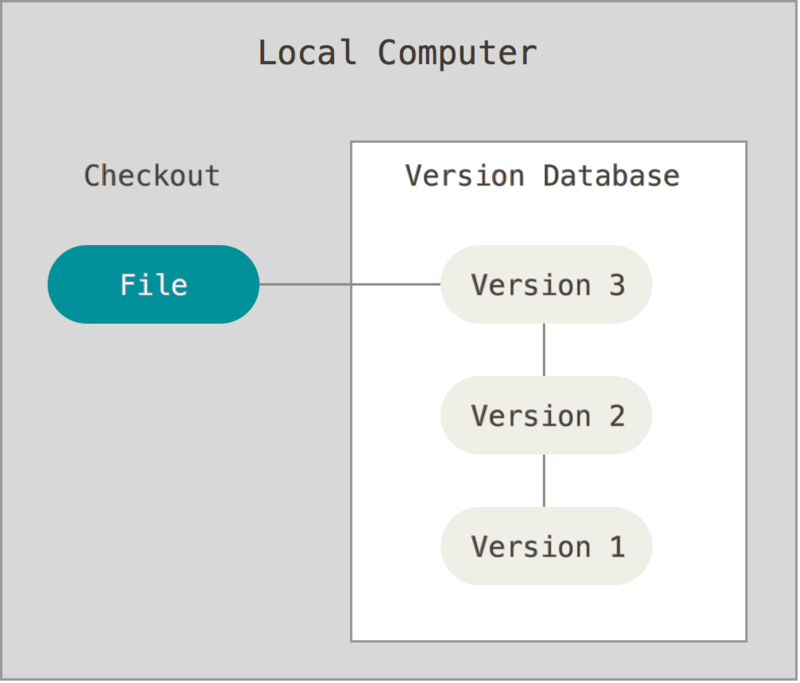
\includegraphics[width=.7\textwidth]{imgs/local.png}
    
        \end{center}
    
    \end{block}

    \textit{Simple database that kept all the changes to files under revision control}

\end{frame}

% sezione intro frame 01
\begin{frame}
    \frametitle{Git and GitHub}
    \framesubtitle{Getting started with Git}
    \addtocounter{nframe}{1}
    
    \begin{block}{Centralized Version Control System}
        \begin{center}

            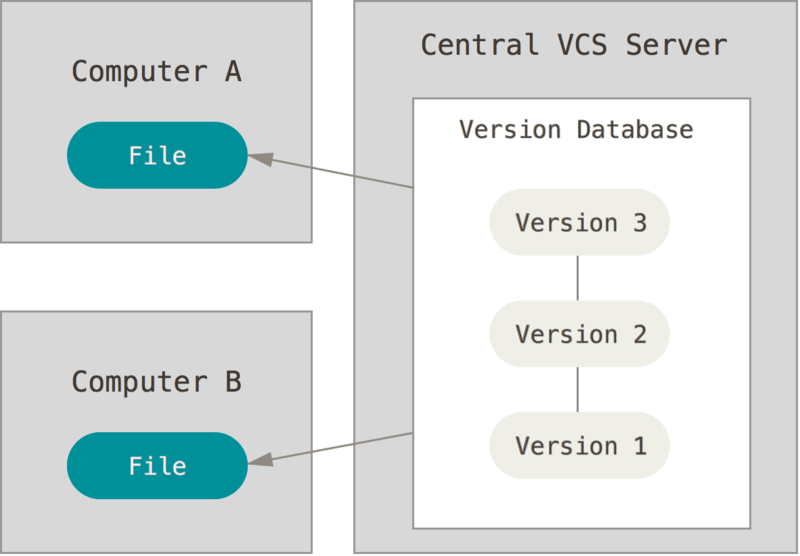
\includegraphics[width=.7\textwidth]{imgs/centralized.png}
    
        \end{center}
    
    \end{block}

    \textit{Need to collaborate: single server that contains all the versioned files}

\end{frame}


% sezione intro frame 01
\begin{frame}
    \frametitle{Git and GitHub}
    \framesubtitle{Getting started with Git}
    \addtocounter{nframe}{1}
    
    \begin{block}{Distributed Version Control System}
        \begin{center}

            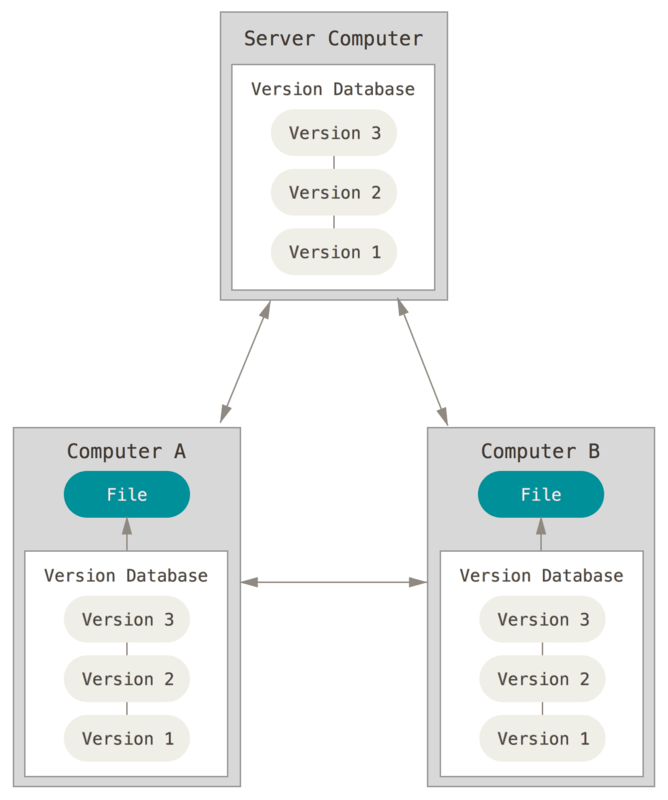
\includegraphics[width=.7\textwidth]{imgs/distributed.png}
    
        \end{center}
    
    \end{block}

    \textit{Client repositories can be copied back up to the server to restore it}

\end{frame}

\begin{frame}
    \frametitle{Git and GitHub}
    \framesubtitle{Getting started with Git}
    \addtocounter{nframe}{1}
    
    \begin{block}{GIT DVCS}
       \begin{itemize}
           \item Started by Linux community
           \item Fast and efficient 
           \item Simple design
           \item non-linear development
           \item fully distributed
           \item handle large projects
           \item easy to use
       \end{itemize}
    
    \end{block}

\end{frame}

\begin{frame}
    \frametitle{Git and GitHub}
    \framesubtitle{Getting started with Git}
    \addtocounter{nframe}{1}
    
    \begin{block}{GIT DVCS}
        With Git, every time you commit, or save the state of your project, Git basically \textbf{takes a picture of what all your files look like} at that moment and stores a \textbf{reference to that snapshot}.    
    \end{block}

\end{frame}

\begin{frame}
    \frametitle{Git and GitHub}
    \framesubtitle{Getting started with Git}
    \addtocounter{nframe}{1}
    
    \begin{block}{GIT DVCS}
        Everything in git is \textbf{checksummed before it is stored} and is then referred to by that checksum
    \end{block}

    \begin{block}{GIT DVCS}
        40-character string composed of hexadecimal characters
    \end{block}
   
    \textit{a62bc012b405ee47d26b695708063a9f2ffad243}

\end{frame}




\begin{frame}
    \frametitle{Git and GitHub}
    \framesubtitle{Getting started with Git}
    \addtocounter{nframe}{1}
    
    \begin{block}{GIT DVCS}
        \begin{center}

            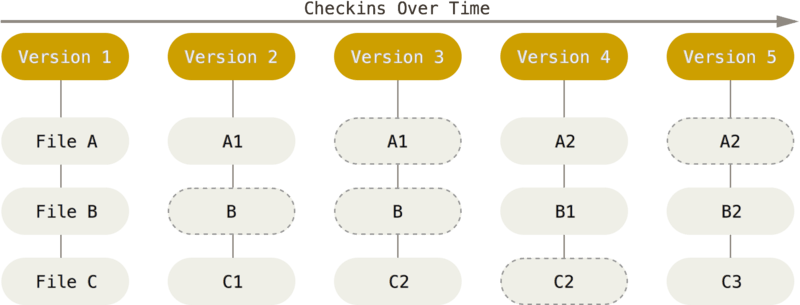
\includegraphics[width=.7\textwidth]{imgs/snapshots-git.png}
    
        \end{center}
    
    \end{block}
    

\end{frame}

\begin{frame}
    \frametitle{Git and GitHub}
    \framesubtitle{Getting started with Git}
    \addtocounter{nframe}{1}
    
    \textbf{Git has three main states that your files can reside in}

    \begin{block}{GIT DVCS}
       \begin{itemize}
           \item committed
           \item modified 
           \item staged
       \end{itemize}
    
    \end{block}

\end{frame}

\begin{frame}
    \frametitle{Git and GitHub}
    \framesubtitle{Getting started with Git}
    \addtocounter{nframe}{1}
    
    \begin{block}{GIT Areas}
        \begin{center}

            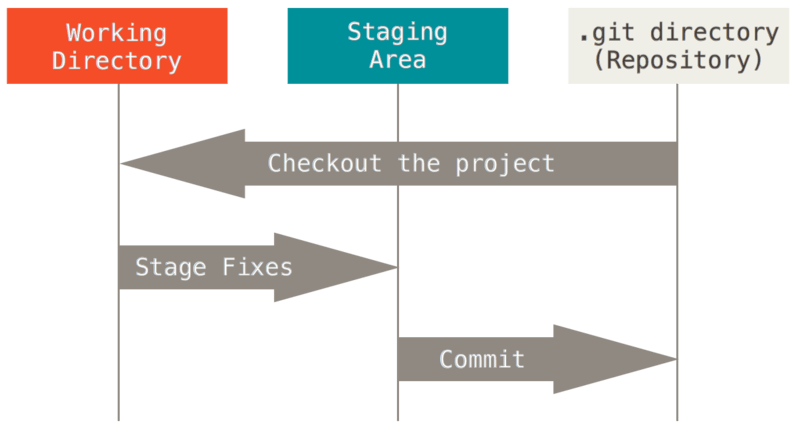
\includegraphics[width=.7\textwidth]{imgs/git-areas.png}
    
        \end{center}
    
    \end{block}
    

\end{frame}

\begin{frame}
    \frametitle{Git and GitHub}
    \framesubtitle{Getting started with Git}
    \addtocounter{nframe}{1}
    
    \textbf{Git has three main states that your files can reside in}

    \begin{block}{GIT local workflow}
       \begin{itemize}
           \item modify files in your working tree
           \item stage just those changes you want to be part of your next commit 
           \item do a commit which stores that snapshot permanently to your git directory
       \end{itemize}
    
    \end{block}

\end{frame}


\section{Git environment by command line interface}
% frame 00
\begin{frame}
	\frametitle{Elementi di Codifica dei Caratteri}
	\framesubtitle{Definizioni}
	\addtocounter{nframe}{1}

	\begin{block}{Rappresentare il testo in formato digitale}
		L’adozione di metodologie informatiche per il trattamento dei testi richiede in primo luogo la disponibilità di un'adeguata rappresentazione dei dati testuali in formato digitale.
	\end{block}

\end{frame}

% frame 00b
\begin{frame}
	\frametitle{Elementi di Codifica dei Caratteri}
	\framesubtitle{Problemi di rappresentazione}
	\addtocounter{nframe}{1}

	\begin{center}
		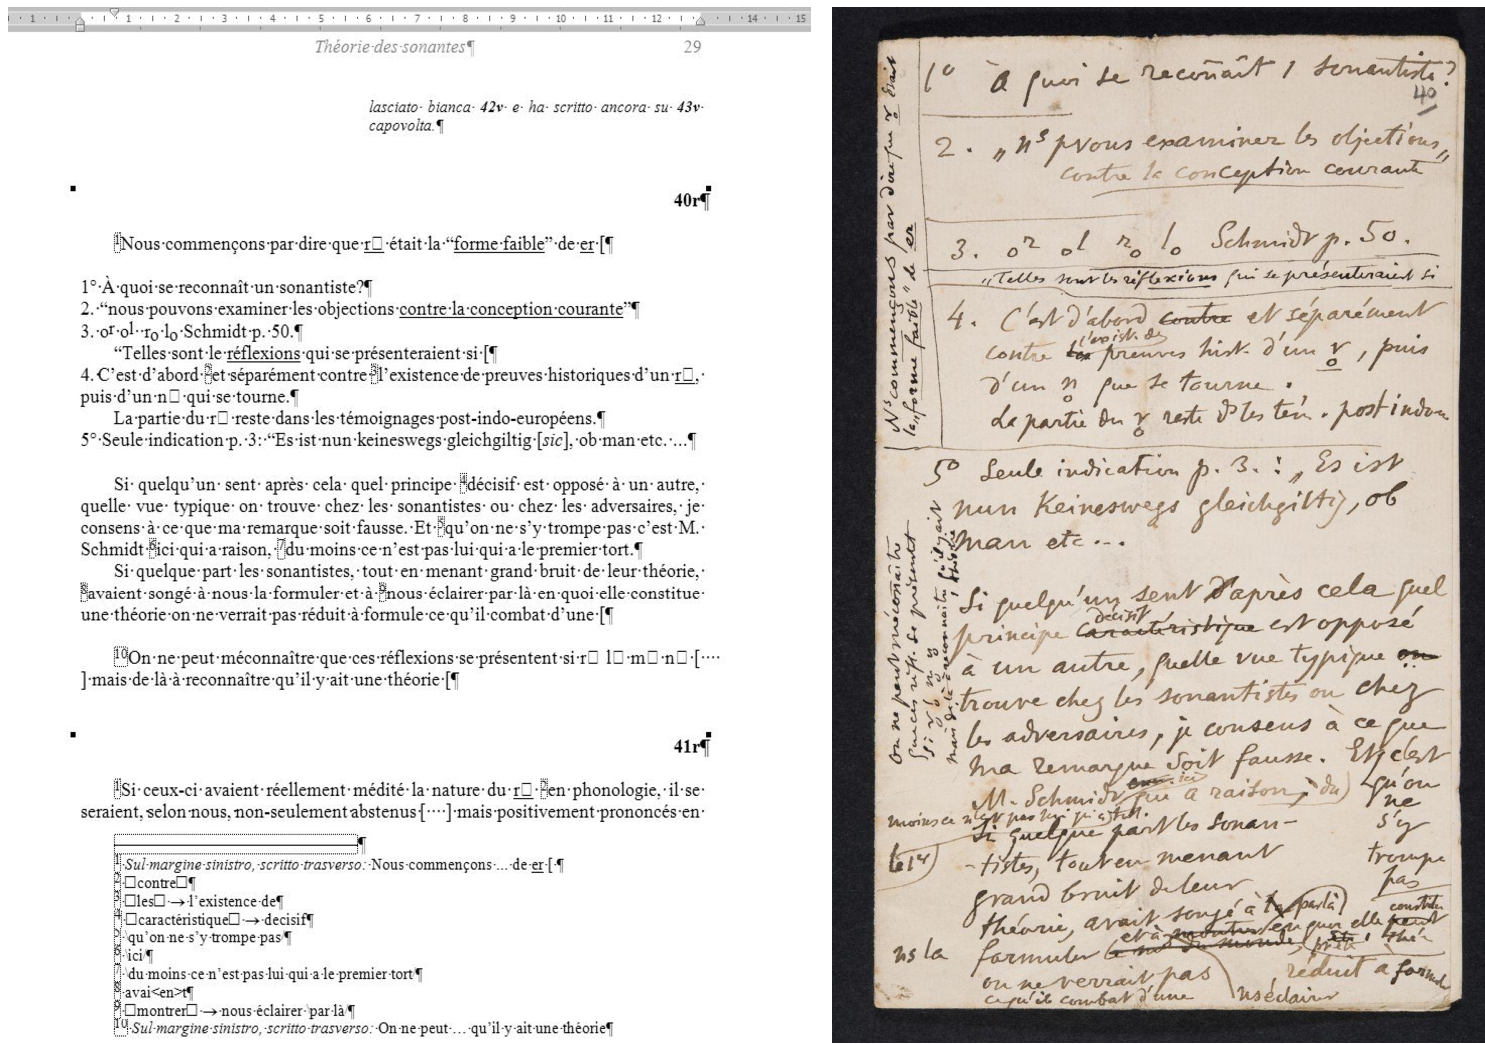
\includegraphics[width=.9\textwidth]{imgs/SaussureTrascrizione.pdf}
	\end{center}

\end{frame}


% frame 01
\begin{frame}
	\frametitle{Elementi di Codifica dei Caratteri}
	\framesubtitle{Definizioni}
	\addtocounter{nframe}{1}

	\begin{block}{Perché è importante la codifica dei caratteri}
		La codifica dei caratteri costituisce il grado zero (basso livello) della rappresentazione di testi su supporto digitale.
		\begin{center}
			\textit{Le codifiche dei caratteri sono la base di qualsiasi schema di codifica testuale}.
		\end{center}
	\end{block}

	\begin{block}{Rappresentazione digitale dei caratteri}
		I caratteri vengono rappresentati all’interno di un elaboratore mediante una sequenza di codici binari formati da opportune disposizioni di cifre composte da 0 e 1: 01100001 \textit{lettera a}
	\end{block}

\end{frame}



% frame 03
\begin{frame}
	\frametitle{Elementi di Codifica dei Caratteri}
	\framesubtitle{American Standard Code for Information Interchange}
	\addtocounter{nframe}{1}

	\begin{block}{Tabella Code Page ASCII 7 bit}
		%immagine di esempio Code Page ASCII (cp1252)
		\begin{center}
			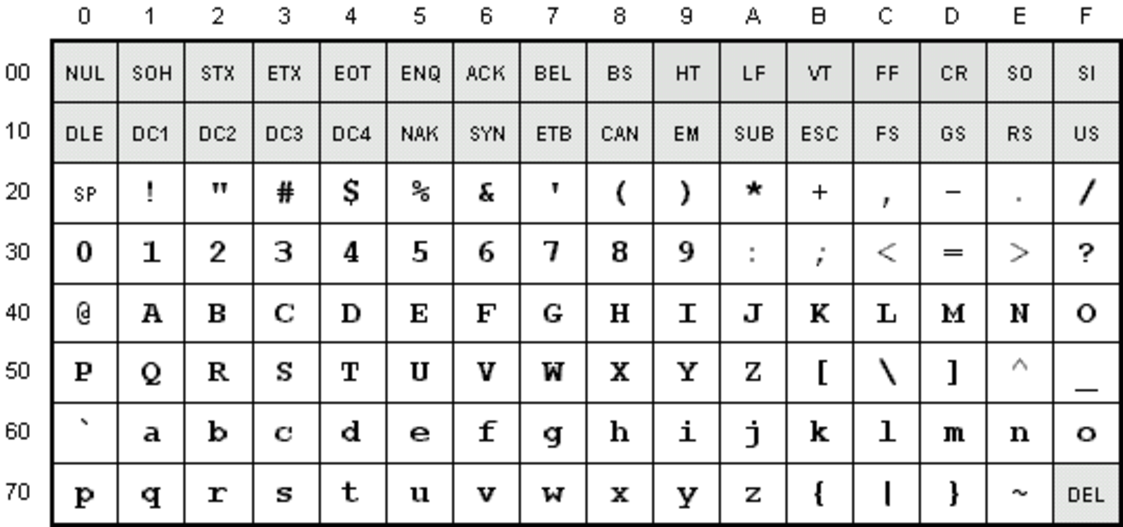
\includegraphics[width=.9\textwidth]{imgs/ascii-67.pdf}
		\end{center}

	\end{block}
	%\hline
	\begin{tiny}
		\begin{center}
			7 bit = 128 possibili caratteri; 32 caratteri di controllo; 96 caratteri effettivi
		\end{center}

	\end{tiny}

\end{frame}

% frame 0
\begin{frame}
	\frametitle{Elementi di Codifica dei Caratteri}
	\framesubtitle{Esempio codifica binaria}
	\addtocounter{nframe}{1}

	\begin{block}{codifica \textit{ciao mondo!} 7 bit ASCII}
		\begin{center}
			\textsc{6369 616f 206d 6f6e 646f 210a}
		\end{center}
	\end{block}

	\begin{block}{codifica \textit{ciao è mondo!} 8 bit ASCII}
		\begin{center}
			\textmd{6369 616f 20\textbf{e8} 206d 6f6e 646f 210a       }
		\end{center}
	\end{block}

	\begin{block}{codifica \textbf{ciao è mondo!} UNICODE UTF-8}
		\begin{center}
			6369 616f 20\textbf{c3 a8}20 6d6f 6e64 6f21 0a
		\end{center}
	\end{block}

\end{frame}

% frame 02
\begin{frame}
	\frametitle{Elementi di Codifica dei Caratteri}
	\framesubtitle{Definizioni}
	\addtocounter{nframe}{1}

	% \begin{block}{Character set, Code Set}
	%  - Character set
	%  - Code Set
	%  - Character encoding
	%  - Tabella del Code page
	% \end{block}

	\begin{description}
		\item [Character Set] Per le discipline che studiano i sistemi di scrittura e l'analisi del linguaggio naturale, un insieme di caratteri astratti è detto Character set (unità alfabetiche). Astratto perché non riguarda la rappresentazione materiale della forma sul supporto, ma è relativo alla forma mentale, fatta di simboli di codifica (referenti).
		\item [Coded Char Set] Per poter trattare un insieme di unità alfabetiche in formato digitale bisogna assegnare a ciascun carattere un numero intero non negativo detto code point.
		
	\end{description}

\end{frame}

% frame 02b
\begin{frame}
	\frametitle{Elementi di Codifica dei Caratteri}
	\framesubtitle{Definizioni}
	\addtocounter{nframe}{1}

	% \begin{block}{Character set, Code Set}
	%  - Character set
	%  - Code Set
	%  - Character encoding
	%  - Tabella del Code page
	% \end{block}

	\begin{description}
		\item [Character Encoding]  Il fine ultimo della codifica è quello di rappresentare una sequenza di caratteri in una sequenza di byte. La codifica di un carattere utilizza uno ``encoding schema'' che a sua volta mappa o trasforma ciascun code point in una sequenza di byte e quindi in ultima istanza in una sequenza di bit. 
		\item [Tabella del code page] Generalmente i code points sono espressi attraverso un sistema numerico esadecimale e disposti in una tabella di associazione.
	\end{description}

\end{frame}

% frame 02c
\begin{frame}
	\frametitle{Elementi di Codifica dei Caratteri}
	\framesubtitle{In sintesi}
	\addtocounter{nframe}{1}


	\begin{block}{Codifica dei caratteri}
		Quindi trasformare una sequenza di caratteri appartenenti ad un char set in una sequenza di byte (bit) significa prima di tutto trasformare/mappare ciascun carattere nel proprio corrispettivo code point e successivamente codificare/serializzare questo code point nella relativa sequenza di byte (bit).
	\end{block}

\end{frame}


% frame 0
\begin{frame}
	\frametitle{Elementi di Codifica dei Caratteri}
	\framesubtitle{Complessità e rappresentazione}
	\addtocounter{nframe}{1}

	\begin{block}{Complessità di rappresentazione universale dei caratteri}
		Se si considerano tutti i possibili alfabeti del mondo e le molteplici esigenze poste dalla scrittura delle fonti manoscritte antiche e medievali, ci si accorge che la realizzazione di un sistema universale per la codifica dei caratteri è un progetto molto complesso con svariate sfide da affrontare.
	\end{block}

\end{frame}

% frame 0
\begin{frame}
	\frametitle{Complessità della Codifica dei Caratteri}
	\framesubtitle{Un Esempio}
	\addtocounter{nframe}{1}

	\begin{center}
		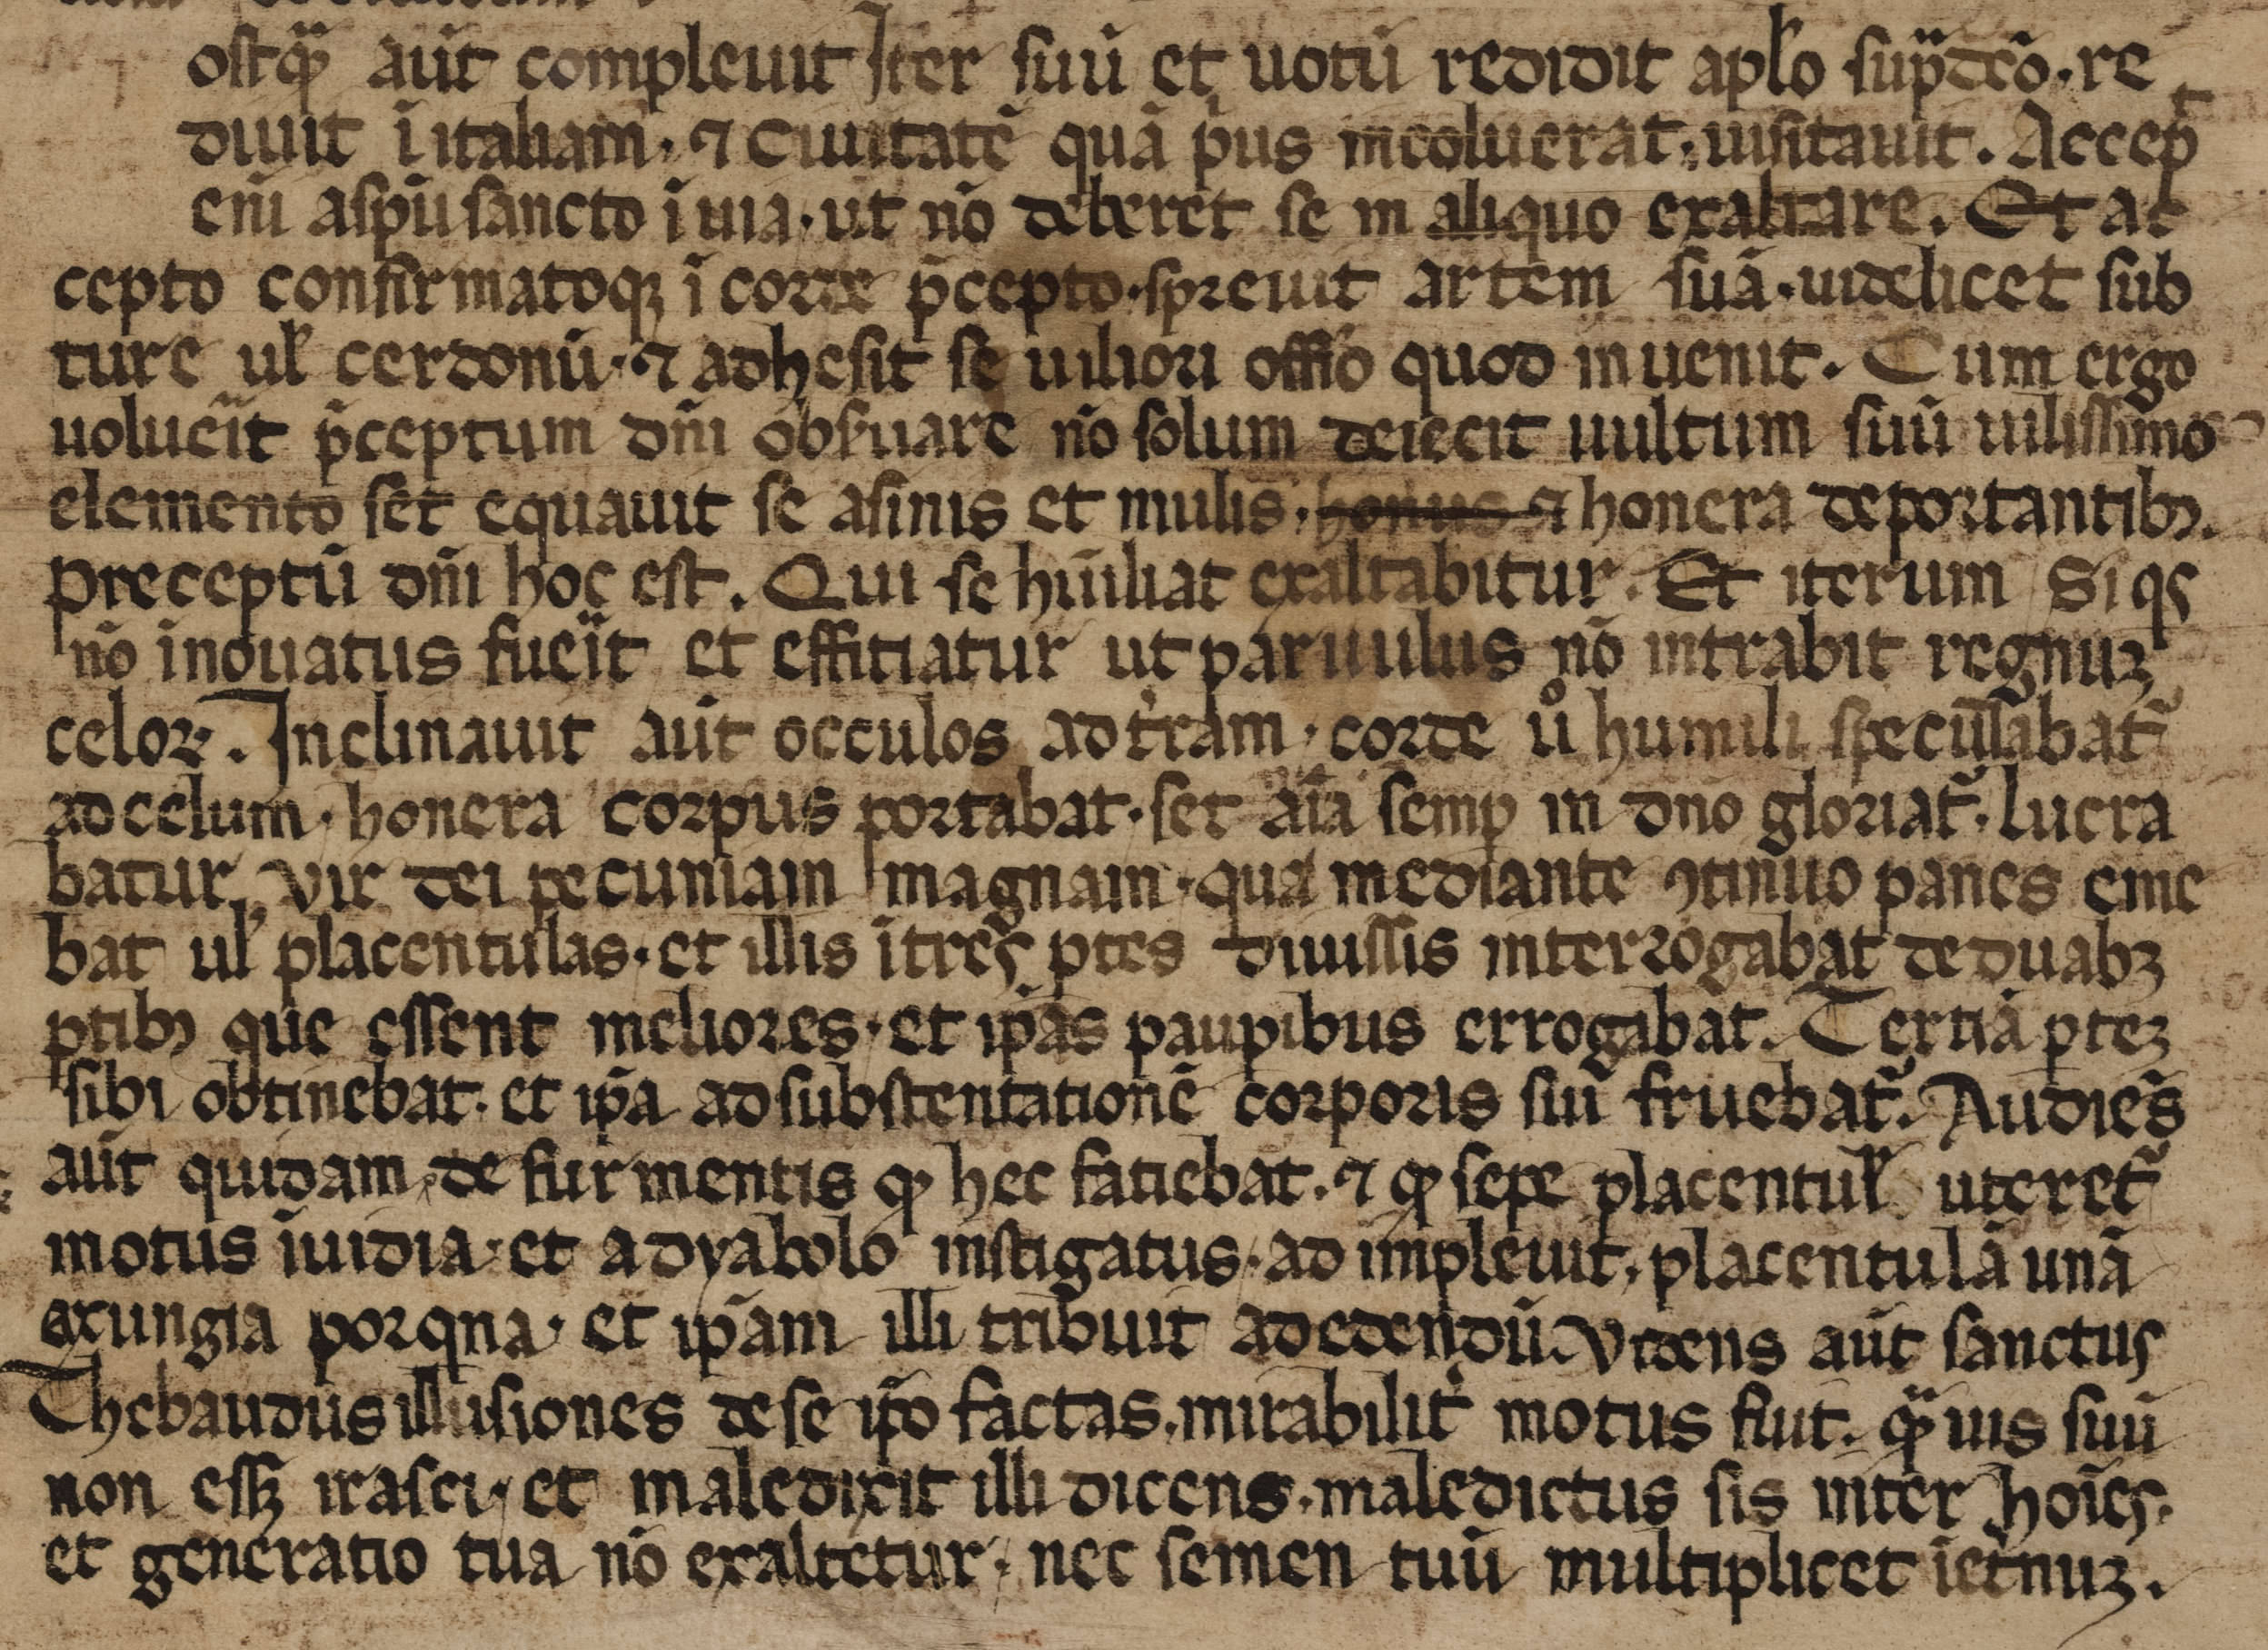
\includegraphics[width=.9\textwidth]{imgs/SnippetRotulo.jpg}
	\end{center}

\end{frame}

% frame 0
\begin{frame}
	\frametitle{Complessità della Codifica dei Caratteri}
	\framesubtitle{Un Esempio}
	\addtocounter{nframe}{1}

	\begin{center}
		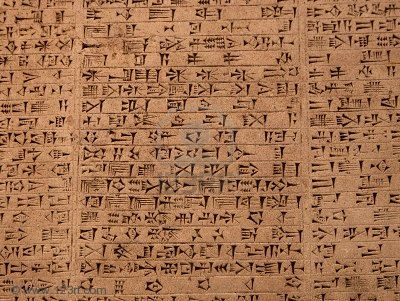
\includegraphics[width=.9\textwidth]{imgs/tavolettaArgilla.jpg}
	\end{center}

\end{frame}


\begin{frame}
	\frametitle{Elementi di Codifica dei Caratteri}
	\framesubtitle{Unicode}
	\addtocounter{nframe}{1}

	\begin{block}{Complessità di rappresentazione universale}
		Ad oggi, lo standard de facto per la codifica dei caratteri è lo UNICODE. Esso è in grado di codificare più di un milione di differenti unità alfabetiche, segni di interpunzione e diacritici, appartenenti a centinaia di diverse lingue.
	\end{block}

	\begin{block}{Complessità di rappresentazione universale}
		%(1.114.111)
		Unicode assegna i propri code point in un range che va da $0x0$ a $0x10FFFF$. In Unicode il code point viene  indicato con una ``U'' seguita da un segno ``+'' seguito a sua volta dall'esadecimale con padding del codice (es: U+0041 lettera A).
	\end{block}

\end{frame}

\begin{frame}
	\frametitle{Elementi di Codifica dei Caratteri}
	\framesubtitle{Unicode}
	\addtocounter{nframe}{1}

	\begin{block}{Unicode Transformation Format}
		Lo Unicode è un Coded Char Set e per essere concretamente serializzato su un supporto elettronico deve essere trasformato attraverso qualche tipo di schema di codifica.
		L'UTF (Unicode Transformation Format) mappa i code point Unicode in sequenze di byte (bit).
	\end{block}

	\begin{block}{UTF standards}
		Esistono tre tipi di schemi di codifica che vanno sotto il nome di UTF, ciascuno è identificato dal minimo numero di bit necessario a codificare ciascun code point: UTF-8; UTF-16; UTF-32. 
	\end{block}

\end{frame}



\section{GitHub host platform}

\begin{frame}
\frametitle{Github}
\framesubtitle{Init a repository}
\addtocounter{nframe}{1}

\begin{block}{Initialization}
	\begin{center}
		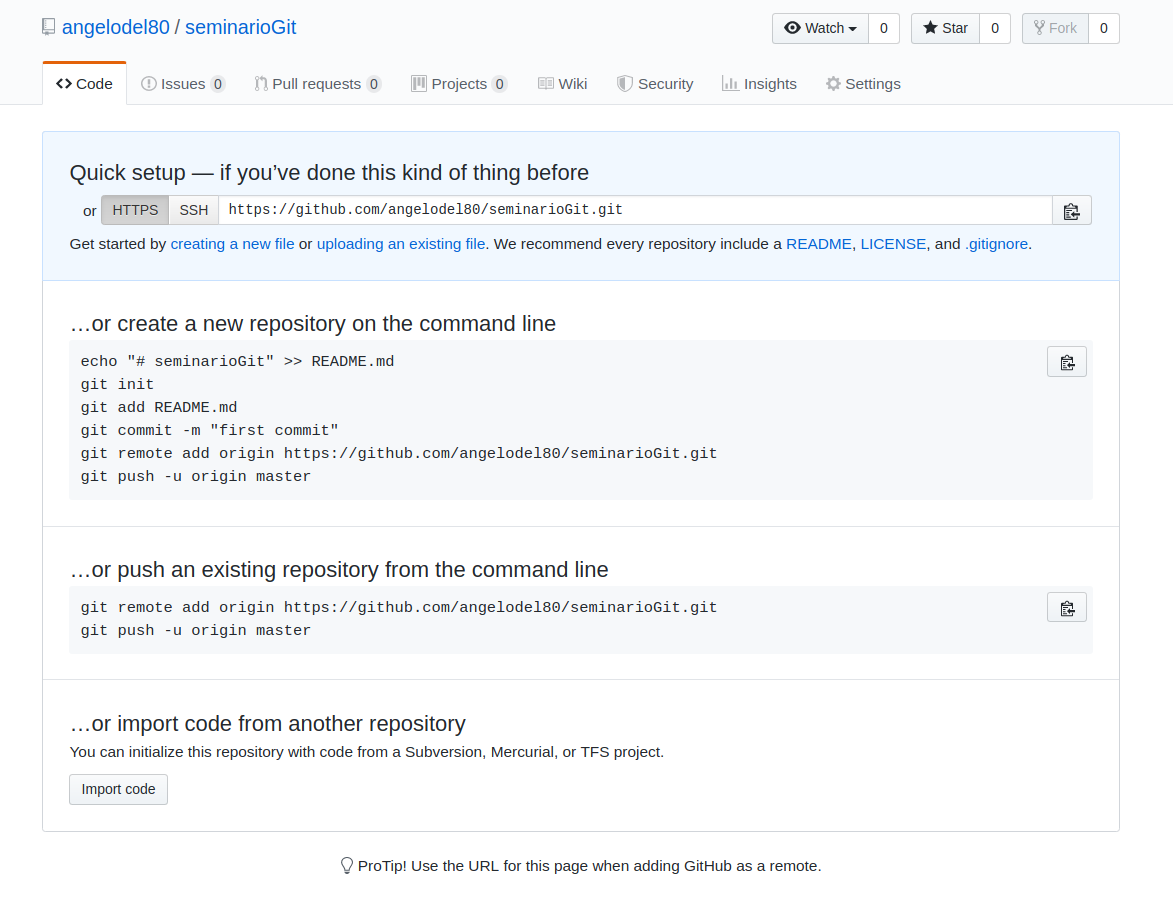
\includegraphics[width=.9\textwidth]{imgs/GitHub-RepoInit.png}
	\end{center}
\end{block}

\end{frame}

\begin{frame}
	\frametitle{Github}
	\framesubtitle{adding collaborators}
	\addtocounter{nframe}{1}
	
	\begin{block}{Formalismi}
		\begin{center}
			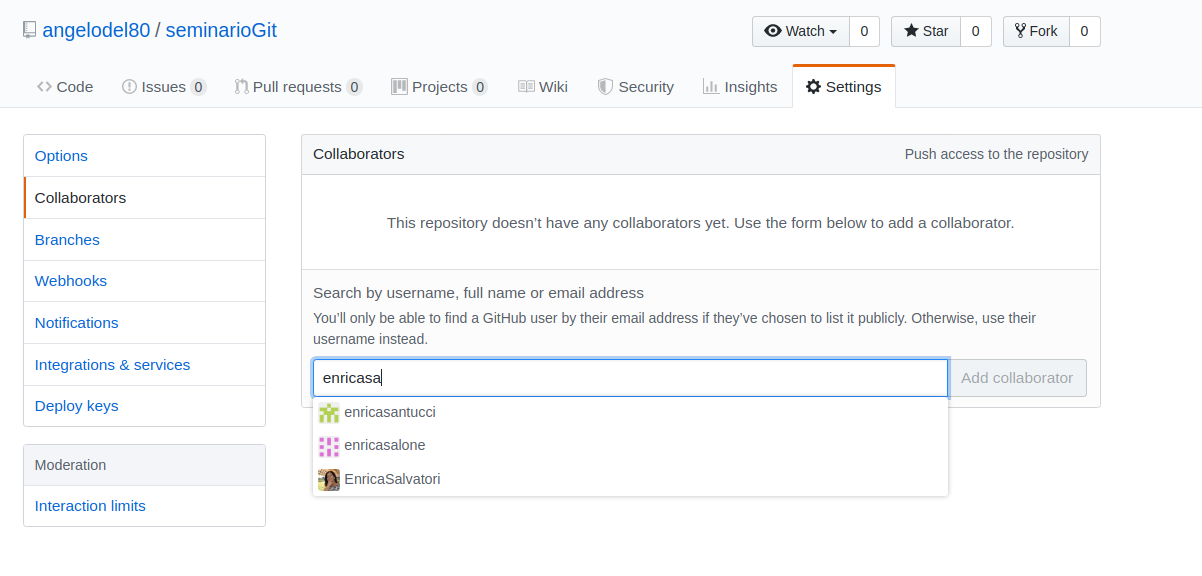
\includegraphics[width=.9\textwidth]{imgs/github-Collaborators.png}
		\end{center}
	\end{block}
	
\end{frame}

\begin{frame}
		\frametitle{Github}
		\framesubtitle{Comments to content lines}
		\addtocounter{nframe}{1}
		
		\begin{block}{Comments}
			\begin{center}
				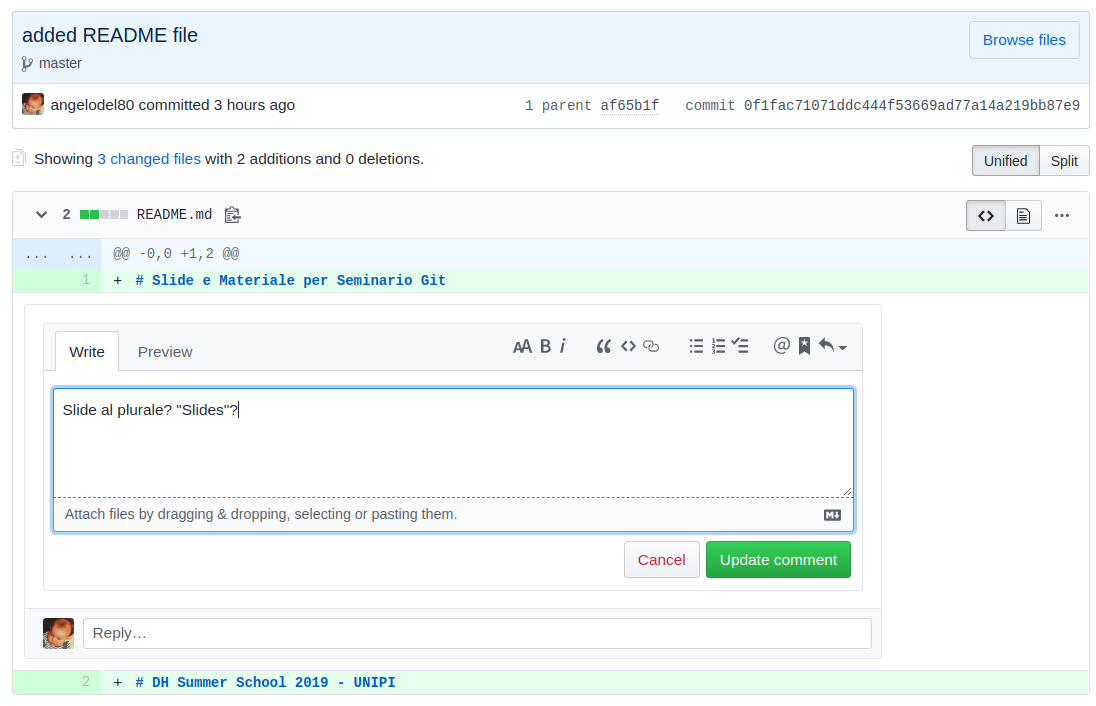
\includegraphics[width=.9\textwidth]{imgs/github-Commento-codice.png}
			\end{center}
		\end{block}

\end{frame}

\begin{frame}
	\frametitle{Github}
	\framesubtitle{Comments to content lines}
	\addtocounter{nframe}{1}
	
	\begin{block}{Comments to comments}
		\begin{center}
			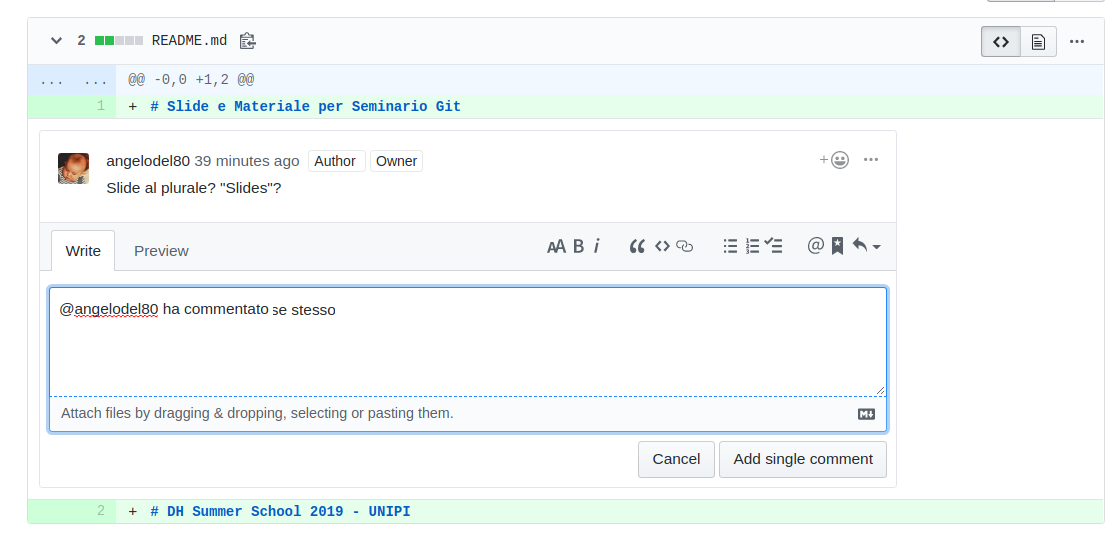
\includegraphics[width=.9\textwidth]{imgs/github-CommentoNotifica.png}
		\end{center}
	\end{block}

\end{frame}
	

\begin{frame}
	\frametitle{Rappresentazione digitale dei testi}
	\framesubtitle{basso e alto livello di codifica}
	\addtocounter{nframe}{1}

	\begin{block}{Codificare un testo}
		La codifica dei caratteri evidentemente non esaurisce i problemi per una opportuna rappresentazione delle caratteristiche interne ed esterne di un testo.
    \end{block}
    
    \begin{block}{Codificare un testo}
		Difatti la codifica del testo è una questione molto più complessa di una semplice riproduzione meccanica di un dato.
	\end{block}


\end{frame}


\begin{frame}
	\frametitle{Rappresentazione digitale dei testi}
	\framesubtitle{basso e alto livello di codifica}
	\addtocounter{nframe}{1}

	\begin{block}{Rappresentare un testo}
		
			La rappresentazione digitale di un testo è una operazione intrinsecamente assai difficile perché coinvolge una pletora di aspetti, a varie dimensioni, a varie granularità e a vari livelli di astrazione sia teorici, sia metodologici, sia tecnologici e sia pratici.
		
	\end{block}

\end{frame}

\begin{frame}
	\frametitle{Rappresentazione digitale dei testi}
	\framesubtitle{basso e alto livello di codifica}
	\addtocounter{nframe}{1}

	\begin{block}{Rappresentare un testo}
		\textbf{
			Prima di poter fare qualsiasi ipotesi su come compiere una codifica di un testo e su come rappresentarlo digitalmente, bisogna stabilire cosa si intende per testo.
		}
	\end{block}

\end{frame}


\begin{frame}
	\frametitle{Rappresentazione digitale dei testi}
	\framesubtitle{Modello dati di un testo}
	\addtocounter{nframe}{1}

	\begin{block}{Un testo non ha una struttura rigida, predefinita: }
		\begin{itemize}

			\item Non è rappresentabile solo come un insieme di record di un archivio elettronico.
			\item Non è rappresentabile solo come un insieme di tabelle di una banca dati.
			\item Non è rappresentabile solo come un albero o un insieme di sotto-alberi
			\item Non è rappresentabile solo come un grafo o come un insieme di sotto grafi

		\end{itemize}

	\end{block}

\end{frame}

\begin{frame}
	\frametitle{Molteplici modelli per diverse esigenze}
	\framesubtitle{Strutture dato e testo}
	\addtocounter{nframe}{1}

	\begin{block}{La rappresentazione di un testo}
		\begin{itemize}
			 %mia slide sulle possibili rappresentazioni del testo
			\item modello lineare: sequenza di dati non strutturati
			\item modello  a record: enumerazione delle proprietà
			\item modello tabulare: insieme di dati omogenei
			\item modello ad albero: gerarchie di dati e insiemi di dati
			\item modello grafo: rete di strutture informative interconnesse tra loro
        \end{itemize}
        
	\end{block}
\end{frame}



\begin{frame}
	\frametitle{Elementi di Codifica del testo}
	\framesubtitle{Formalismi}
	\addtocounter{nframe}{1}

	\begin{block}{Formati di rappresentazione}
		\begin{center}
			Un formato è un insieme di regole e convenzioni formali per rappresentare un insieme di dati, nel nostro caso un testo.
		\end{center}

	\end{block}

	\begin{block}{Importanza dei formati}
		\begin{center}
			Seppur isomorfi la scelta dei formati condiziona molto l'efficienza delle operazioni e l'efficacia delle dichiarazioni.
		\end{center}

	\end{block}


\end{frame}

%\begin{frame}
%    \frametitle{Elementi di Codifica del testo}
%    \framesubtitle{lista di formati}
%    \addtocounter{nframe}{1}
%   
%    \begin{block}{Formati dato}
%Data structures – CSV and tabular data
%– JSON
%– RDF
%Plain text formats – Plain text
%– TeX, LaTeX, etc.
%– Markdown, CommonMark and wiki syntaxes
%Markup formats
%– HTML, HTML5
%– XML
%– HTML5+ Embedded annotations (e.g., HTML5 + RDFa)
%– Markup spinoffs for overlapping (e.g. LMNL, TexMECS, etc.) 
%
%    \end{block}

% \begin{block}{Riferimenti TEI}
%     Capitolo sul character encoding e modulo Ganji 
% \end{block}

%\end{frame}

\begin{frame}
	\frametitle{Elementi di Codifica del testo}
	\framesubtitle{Tabella Formalismi}
	\addtocounter{nframe}{1}

	\begin{block}{Formalismi}
		\begin{center}
			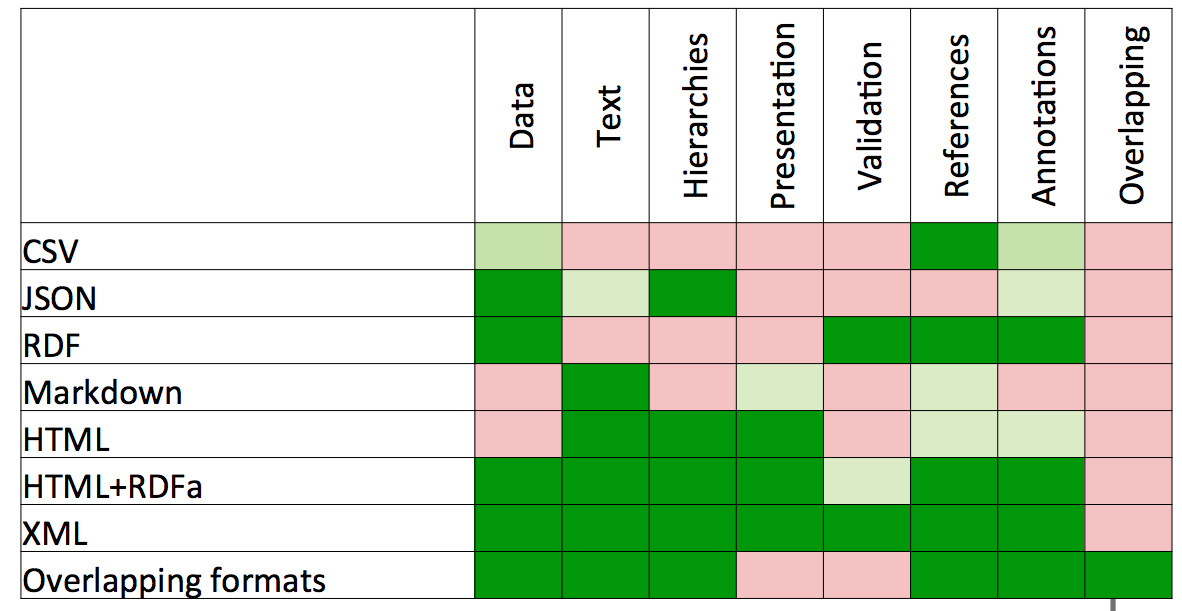
\includegraphics[width=.9\textwidth]{imgs/TabellaFormalismiCodificaTesto.png}
		\end{center}
	\end{block}
	courtesy of \textit{Fabio Vitali}

\end{frame}


\begin{frame}
	\frametitle{Elementi di Codifica del testo}
	\framesubtitle{Varietà di rappresentazione}
	\addtocounter{nframe}{1}

	
		\begin{center}
			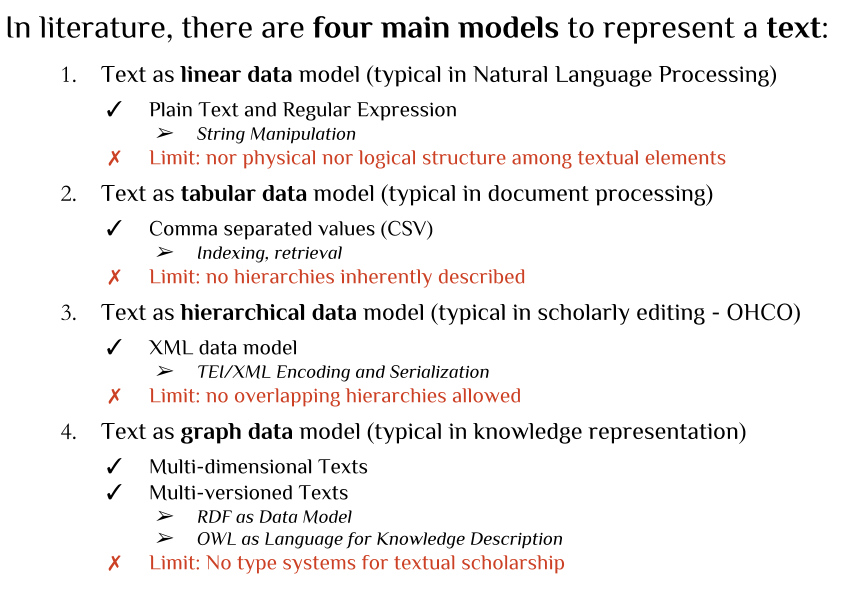
\includegraphics[width=.9\textwidth]{imgs/dataModels-slide.png}
		\end{center}
	
	
\end{frame}

\begin{frame}
	\frametitle{Elementi di Codifica del testo}
	\framesubtitle{Esempio di codifica del testo utilizzando CSV}
	\addtocounter{nframe}{1}

		
			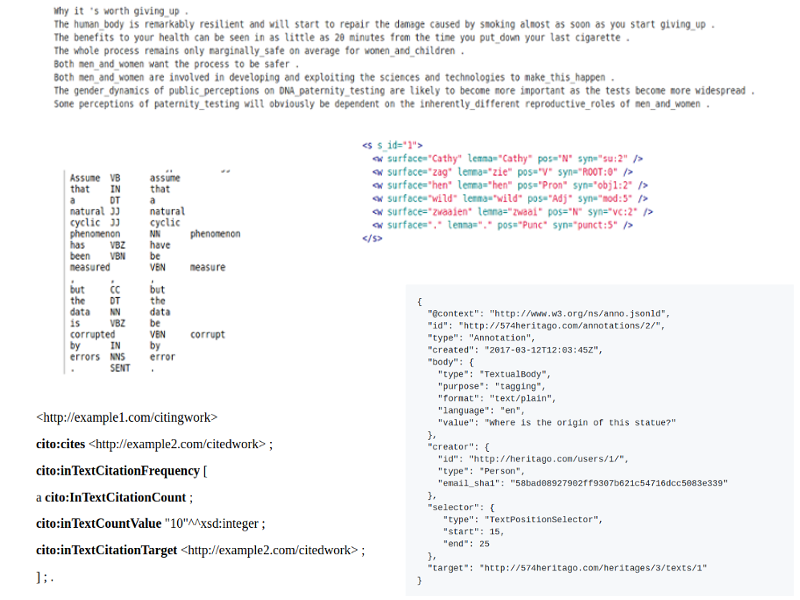
\includegraphics[width=1.1\textwidth]{imgs/VariRappresentazioniTesto.png}
		
	
\end{frame}



\begin{frame}
	\frametitle{Elementi di Codifica del testo}
	\framesubtitle{Formalismi}
	\addtocounter{nframe}{1}

	\begin{block}{Formati come formalismi}
		\begin{center}
			Data l'importanza metodologica il formato del dato diviene un vero e proprio formalismo, si parla cioè di linguaggi di codifica in quanto questi sistemi si basano su un insieme di istruzioni rigorose di codifica.
		\end{center}

	\end{block}

\end{frame}



\begin{frame}
	\frametitle{Elementi di Codifica del testo}
	\framesubtitle{Formalismi}
	\addtocounter{nframe}{1}

	\begin{block}{Formati e formalismi di codifica}

		Quindi ogni pezzo di informazione aggiunta ad un testo grezzo attraverso l'inserimento di dati metatestuali (markup, annotazione, codifica), constituisce il risultato di una analisi e di una interpretazione che è stata condotta (da un umano o da una macchina) al fine di esplicitare e rappresentare nel modo più accurato e completo possibile le informazioni da veicolare attraverso il formato digitale prescelto (anche in modo incrementale).


	\end{block}

\end{frame}





% % altra slide Vitali
% • Text has characters, including punctuation
% – We all (sort of) agree on this
% • Texts is ordered
% – In ``To be or not to be'', it is important that ``To be''
% comes before ``not to be''
% • Text has structure
% • Text has presentation
% • Text has grammar
% • Texts has semantics
% • Text has variants
% • Text has a lot of things that can be said about it 

% • Evidenziazione, page 170
% GitHub is the single largest host for Git repositories,

% • Evidenziazione, page 170
% central point of collaboration

% • Evidenziazione, page 170
% A large percentage of all Git repositories are hosted on GitHub

% • Evidenziazione, page 170
% Git hosting, issue tracking, code review, and other things

% • Evidenziazione, page 170
% need to interact with GitHub at some point while using Git professionally

% • Evidenziazione, page 170
% This chapter is about using GitHub effectively.

% • Evidenziazione, page 170
% signing up for and managing an account

% • Evidenziazione, page 170
% creating and using Git repositories, common workflows to contribute to projects and to accept contributions to yours

% • Evidenziazione, page 170
% set up a free user account

% • Evidenziazione, page 170
% Sign up for GitHub

% • Evidenziazione, page 171
% GitHub will send you an email to verify the address you provided

% • Evidenziazione, page 171
% your dashboard page

% • Evidenziazione, page 171
% ready to use GitHub

% • Evidenziazione, page 171
% connect with Git repositories using the https:// protocol

% • Evidenziazione, page 172
% Next, if you wish, you can replace the avatar that is generated for you with an image of your choosing.

% • Evidenziazione, page 173
% people will see your avatar next to your username

% • Evidenziazione, page 174
% The way that GitHub maps your Git commits to your user is by email address

% • Evidenziazione, page 174
% extra security

% • Evidenziazione, page 174
% Two-factor Authentication

% • Evidenziazione, page 174
% Authentication is an authentication mechanism

% • Evidenziazione, page 175
% code in addition to your password whenever you log into GitHub.

% • Evidenziazione, page 175
% could be useful in helping you contribute to an existing project

% • Evidenziazione, page 175
% you don’t have push access, you can “fork” the project

% • Evidenziazione, page 175
% GitHub will make a copy of the project that is entirely yours

% • Evidenziazione, page 175
% it lives in your namespace, and you can push to it

% • Evidenziazione, page 175
% 170 about the change until the owner is happy with it

% • Evidenziazione, page 175
% In GitHub, a “fork” is simply the same project in your own namespace

% • Evidenziazione, page 175
% People can fork a project, push to it, and contribute their changes back to the original repository by creating what’s called a Pull Request

% • Evidenziazione, page 175
% This opens up a discussion thread with code review,

% • Evidenziazione, page 175
% the contributor can then communicate 170 about the change until the owner is happy with it

% • Evidenziazione, page 176
% at which point the owner can merge it in

% • Evidenziazione, page 176
% “Fork” button

% • Evidenziazione, page 176
% with your own writeable copy of the code.

% • Evidenziazione, page 176
% GitHub is designed around a particular collaboration workflow, centered on Pull Requests.

% • Evidenziazione, page 176
% teams use GitHub’s web based tools.

% • Evidenziazione, page 176
% Let’s walk through an example

% • Evidenziazione, page 177
% So let’s improve the program and submit it back to the project as a proposed change.

% • Evidenziazione, page 177
% we click the Fork button as mentioned earlier to get our own copy of the project.

% • Evidenziazione, page 177
% We will clone it locally, create a topic branch, make the code change and finally push that change back up to GitHub.

% • Evidenziazione, page 178
% git diff --word-diff

% • Evidenziazione, page 178
% [-delay(1000);-]{+delay(3000);+}

% • Evidenziazione, page 178
% [-delay(1000);-]{+delay(3000);+}

% • Evidenziazione, page 178
% Clone our fork of the project locally

% • Evidenziazione, page 178
% Create a descriptive topic branch

% • Evidenziazione, page 178
% Make our change to the code

% • Evidenziazione, page 178
% Check that the change is good

% • Evidenziazione, page 178
% Commit our change to the topic branch

% • Evidenziazione, page 178
% Push our new topic branch back up to our GitHub fork

% • Evidenziazione, page 178
% GitHub noticed that we pushed a new

% • Evidenziazione, page 179
% topic branch up and presents us with a big green button

% • Evidenziazione, page 179
% check out our changes and open a Pull Request to the original project

% • Evidenziazione, page 179
% give our Pull Request a title and description.

% • Evidenziazione, page 179
% unified diff of all the changes that will be made should this branch get merged by the project owner

% • Evidenziazione, page 180
% Create pull request button

% • Evidenziazione, page 180
% it’s also often used in internal projects at the beginning of the development cycle

% • Evidenziazione, page 180
% the project owner can look at the suggested change and merge it

% • Evidenziazione, page 180
% reject it or comment on it

% • Evidenziazione, page 181
% on GitHub this happens online

% • Evidenziazione, page 181
% leave a comment by clicking on any of the lines

% • Evidenziazione, page 181
% Anyone can also leave general comments on the Pull Request.

% • Evidenziazione, page 181
% both commenting on a line of code

% • Evidenziazione, page 181
% leaving a general comment in the discussion section

% • Evidenziazione, page 182
% with GitHub you simply commit to the topic branch again and push, which will automatically update the Pull Request

% • Evidenziazione, page 182
% Adding commits to an existing Pull Request doesn’t trigger a notification

% • Evidenziazione, page 183
% This button only shows up if you have write access to the repository and a trivial merge is possible

% • Evidenziazione, page 183
% If you click it GitHub will perform a “non-fast-forward” merge, meaning that even if the merge could be a fast-forward, it will still create a merge commit.

% • Evidenziazione, page 184
% This is the basic workflow that most GitHub projects use

% • Evidenziazione, page 184
% Topic branches are created, Pull Requests are opened on them, a discussion ensues, possibly more work is done on the branch and eventually the request is either closed or merged.

% • Evidenziazione, page 184
% initiate the code review and discussion process

% • Evidenziazione, page 184
% No forking necessary

% • Evidenziazione, page 195
% creating, maintaining and administering your own project.

% • Evidenziazione, page 195
% Let’s create a new repository to share our project code with

% • Evidenziazione, page 197
% All you really have to do here is provide a project name;

% • Evidenziazione, page 197
% click the “Create Repository” button

% • Evidenziazione, page 197
% new repository on GitHub,

% • Evidenziazione, page 197
% Since you have no code there yet, GitHub will show you instructions for how to create a brand-new Git repository, or connect an existing Git project.

% • Evidenziazione, page 197
% Now that your project is hosted on GitHub, you can give the URL to anyone you want to share your project with.

% • Evidenziazione, page 197
% It is often preferable to share the HTTPS based URL for a public project

% • Evidenziazione, page 197
% The HTTPS one is also exactly the same URL they would paste into a browser to view the project there.

% • Evidenziazione, page 197
% If you’re working with other people who you want to give commit access to, you need to add them as “collaborators”

% • Evidenziazione, page 197
% you want to give them push access to your repository, you can add them to your project.

% • Evidenziazione, page 197
% “push” access

% • Evidenziazione, page 197
% both read and write access to the project and Git repository

% • Evidenziazione, page 198
% Then select “Collaborators”

% • Evidenziazione, page 198
% You can repeat this as many times as you like to grant access to everyone you like

% • Evidenziazione, page 198
% revoke access, just click the “X”

% • Evidenziazione, page 198
% get a Pull Request yourself.

% • Evidenziazione, page 198
% Pull Requests can either come from a branch in a fork of your repository or they can come from another branch in the same repository.

% • Evidenziazione, page 198
% The only difference is that the ones in a fork are often from people where you can’t push to their branch and they can’t push to yours,

% • Evidenziazione, page 198
% with internal Pull Requests generally both parties can access the branch.

% • Evidenziazione, page 199
% The other interesting URLs are the .diff and .patch URLs, which as you may guess, provide unified diff and patch versions of the Pull Request.

% • Evidenziazione, page 200
% As we covered in The GitHub Flow, you can now have a conversation with the person who opened the Pull Request.

% • Evidenziazione, page 200
% comment on specific lines of code

% • Evidenziazione, page 200
% Once the code is in a place you like and want to merge it in, you can either pull the code down and merge it locally, either with the git pull <url> <branch> syntax we saw earlier, or by adding the fork as a remote and fetching and merging.

% • Evidenziazione, page 201
% If you decide you don’t want to merge it, you can also just close the Pull Request and the person who opened it will be notified.

% • Evidenziazione, page 201
% neat trick tha

% • Evidenziazione, page 203
% If you see a Pull Request that is moving in the right direction and you have an idea for a change that depends on it or you’re not sure is a good idea, or you just don’t have push access to the target branch, you can open a Pull Request directly to it.

% • Evidenziazione, page 204
% Mentions and Notifications

% • Evidenziazione, page 204
% GitHub also has a pretty nice notifications system

% • Evidenziazione, page 204
% In any comment you can start typing a @ character and it will begin to autocomplete with the names and usernames of people who are collaborators or contributors in the project.

% • Evidenziazione, page 204
% pulling people into conversations rather than making them poll

% • Evidenziazione, page 205
% You will also be subscribed to something if you opened it, if you’re watching the repository or if you comment on something

% • Evidenziazione, page 205
% no longer wish to receive notifications, there is an “Unsubscribe” button

% • Evidenziazione, page 205
% If you go to the “Notification center” tab from the settings page, you can see some of the options you have.

% • Evidenziazione, page 206
% The two choices are to get notifications over “Email” and over “Web” and you can choose either,

% • Evidenziazione, page 206
% Web notifications only exist on GitHub and you can only check them on GitHub

% • Evidenziazione, page 206
% If you click on that, you will see a list of all the items you have been notified about

% • Evidenziazione, page 207
% Email notifications are the other way you can handle notifications through GitHub

% • Evidenziazione, page 207
% It’s also worth noting that if you have both email and web notifications enabled and you read the email version of the notification, the web version will be marked as read as well if you have images allowed in your mail client.

% • Evidenziazione, page 207
% There are a couple of special files that GitHub will notice if they are present in your repository.

% • Evidenziazione, page 208
% The first is the README file, which can be of nearly any format that GitHub recognizes as prose. For example, it could be README, README.md, README.asciidoc, etc. If GitHub sees a README file in your source, it will render it on the landing page of the project.

% • Evidenziazione, page 208
% Many teams use this file to hold all the relevant project information for someone who might be new to the repository or project. This generally includes things like:

% • Evidenziazione, page 208
% What the project is for

% • Evidenziazione, page 208
% How to configure and install it

% • Evidenziazione, page 208
% An example of how to use it or get it running

% • Evidenziazione, page 208
% The license that the project is offered under

% • Evidenziazione, page 208
% How to contribute to it

% • Evidenziazione, page 208
% Since GitHub will render this file, you can embed images or links in it for added ease of understanding.

% • Evidenziazione, page 208
% Generally there are not a lot of administrative things you can do with a single project, but there are a couple of items that might be of interest.

% • Evidenziazione, page 209
% If you would like to transfer a project to another user or an organization in GitHub, there is a “Transfer ownership” option at the bottom of the same “Options” tab of your repository settings page that allows you to do this.

% • Evidenziazione, page 209
% This is helpful if you are abandoning a project and someone wants to take it over

% • Evidenziazione, page 209
% move it into an organization.

% • Evidenziazione, page 209
% sets up a redirect from your URL

% • Evidenziazione, page 210
% In addition to single-user accounts, GitHub has what are called Organizations

% • Evidenziazione, page 210
% Organizational accounts have a namespace where all their projects exist

% • Evidenziazione, page 210
% These accounts represent a group of people with shared ownership of projects

% • Evidenziazione, page 210
% many tools to manage subgroups of those people

% • Evidenziazione, page 210
% companies

% • Evidenziazione, page 210
% New organization” from the menu

% • Evidenziazione, page 210
% First you’ll need to name your organization and provide an email address for a main point of contact for the group

% • Evidenziazione, page 210
% When you create new repositories you can create them either under your personal account or under any of the organizations that you are an owner in

% • Evidenziazione, page 210
% Organizations are associated with individual people by way of teams

% • Evidenziazione, page 210
% grouping of individual user accounts and repositories within the organization

% • Evidenziazione, page 211
% Teams make this easy, without having to manage the collaborators for every individual repository.

% • Evidenziazione, page 211
% ou can use to add members to the team

% • Evidenziazione, page 211
% Each team can have read only, read/write or administrative access to the repositorie

% • Evidenziazione, page 211
% “Settings” button

% • Evidenziazione, page 212
% Additionally, team @mentions (such as @acmecorp/frontend) work much the same as they do with individual users, except that all members of the team are then subscribed to the thread

% • Evidenziazione, page 212
% Organizations also give owners access to all the information about what went on under the organization. You can go to the Audit Log tab and see what events have happened at an organization level, who did them and where in the world they were done.

% • Evidenziazione, page 220
% curl

% • Evidenziazione, page 222
% GitHub user

% • Evidenziazione, page 222
% how to create an account

% • Evidenziazione, page 222
% manage an organization,

% • Evidenziazione, page 222
% create and push to repositories

% • Evidenziazione, page 222
% contribute to other people’s projects

% • Evidenziazione, page 222
% ccept contributions from others

% • Evidenziazione, page 223
% ource code control

% • Evidenziazione, page 223
% basic tasks of tracking and committing files

% • Evidenziazione, page 360
% important actions occur

%\section{Extra}
%% sezione XML frame 01
\begin{frame}
	\frametitle{Codifica ad alto livello}
	\framesubtitle{Sistemi di marcatura}
	\addtocounter{nframe}{1}

	\begin{block}{Metodi e tecniche per la codifica di testi}
		La riflessione sui metodi e le pratiche migliori per la codifica elettronica dei testi è stato uno dei temi fondamentali della ricerca e della sperimentazione nel dominio dell’Informatica umanistica per molti anni.
	\end{block}

\end{frame}

% sezione XML frame 02
\begin{frame}
	\frametitle{Markup language e XML}
	\framesubtitle{soluzione corrente per la codifica dei testi}
	\addtocounter{nframe}{1}

	\begin{block}{XML per la descrizione e la codifica}
		Ad oggi la soluzione considerata ottimale per una corretta rappresentazione del testo è l'adozione dei markup language descrittivi basati su XML.
	\end{block}

	\begin{block}{TEI-XML}
		Standard de facto per la codifica dei testi è considerato lo schema XML messo a punto dalla Text Encoding Initiative (TEI-XML).
	\end{block}

\end{frame}

% sezione XML frame 02b
\begin{frame}
	\frametitle{Lo schema TEI-XML}
	\framesubtitle{Estratto di documento TEI-XML}
	\addtocounter{nframe}{1}

	\begin{center}
		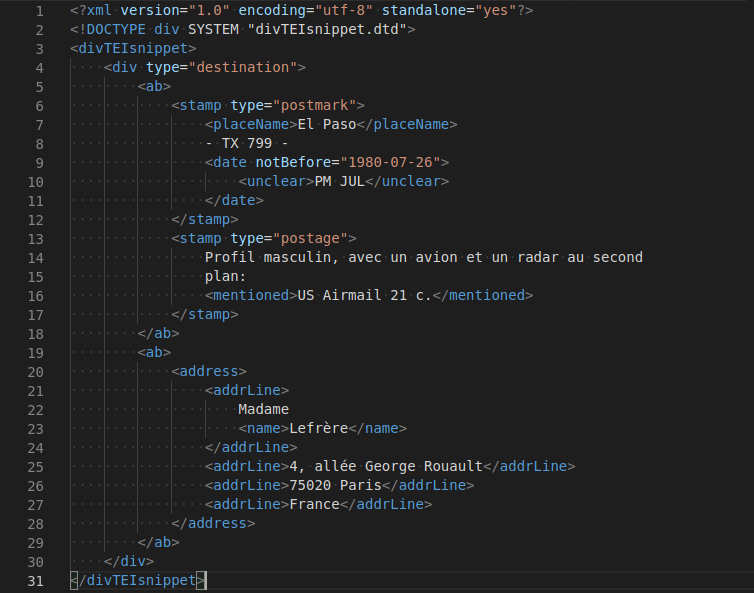
\includegraphics[width=.9\textwidth]{imgs/DivTEISnippet.png}
	\end{center}
	
\end{frame}

% sezione XML frame 02c
\begin{frame}
	\frametitle{TEI-XML}
	\framesubtitle{Motivazioni per adottare TEI}
	\addtocounter{nframe}{1}

	\begin{block}{Perché TEI}
		La Text Encoding Initiative (TEI) è un autorevole progetto internazionale, a cui afferiscono varie organizzazioni e università, il cui scopo è fornire agli studiosi di informatica umanistica uno strumento il più espressivo e flessibile possibile per rappresentare qualsiasi aspetto di interesse relativo alla risorsa testuale da rappresentare digitalmente.
	\end{block}

\end{frame}

% sezione XML frame 03
\begin{frame}
	\frametitle{Impiego di XML}
	\framesubtitle{Benefici}
	\addtocounter{nframe}{1}

	\begin{block}{Perché XML}
		\begin{itemize}
			\item separazione dei dati dall'applicativo di authoring/editing 
			\item separazione della rappresentazione dei dati dalla presentazione dei dati
			\item possibilità di trasformare i dati in qualsiasi altro formato compatibile
			\item leggibilità dei documenti XML da parte di esseri umani
		\end{itemize}

	\end{block}
	

\end{frame}

% sezione XML frame 03b
\begin{frame}
	\frametitle{Impiego di XML}
	\framesubtitle{Benefici}
	\addtocounter{nframe}{1}

	\begin{block}{Perché XML}
		\begin{itemize}
			\item standard w3c testuale, aperto, personalizzabile e liberamente utilizzabile
			\item semplicità di condivisione e scambio dati (interoperabilità e portabilità)
			\item adatto per codificare dati semistrutturati oltre che a dati strutturati
			\item validazione del documento attraverso spcificazioni formali
		\end{itemize}

	\end{block}
	

\end{frame}


% sezione XML frame 04
\begin{frame}
	\frametitle{Ecosistema XML}
	\framesubtitle{Le tecnologie XML per la definizione ed elaborazione di documenti XML}
	\addtocounter{nframe}{1}

	\begin{itemize}
		\item XSD: XML Schema Definition Language
		\item XPath: XML Path Language
		\item XSL: eXtensible Stylesheet Language
		\item XSL-T:  XSL – Transformations
		\item XSL-FO: XSL – Formatting Objects
		\item XQuery: XML Query Language for XML Databases
		\item XInclude: XML inclusion Language
		\item DTD: Document Type Definition Language
		\item RelaxNG: Regular Expression Language for XML (New Generation)
	\end{itemize}

\end{frame}


% sezione XML frame 05
\begin{frame}
	\frametitle{Linguaggio di marcatura XML}
	\framesubtitle{}
	\addtocounter{nframe}{1}

	\begin{block}{Perché XML}
		Adottando la tecnologia e il linguaggio XML abbiamo la possibilità di creare linguaggi di marcatura personalizzati e specifici per ogni esigenza e dominio.
	\end{block}

\end{frame}

\begin{frame}
	\frametitle{XML come linguaggio per la codifica di testi}
	\framesubtitle{}
	\addtocounter{nframe}{1}

	\begin{block}{Vantaggi}
		Attraverso XML è possibile strutturare i dati, gestire in modo nativo strutture gerarchiche, elaborare e presentare i dati con strumenti XML nativi, validare i tipi di strutture e i tipi di dati consentiti, gestire riferimenti incrociati tramite opportuni meccanismi di dereferenziazione, aggiungere e gestire annotazioni a vari livelli di granularità.
	\end{block}


\end{frame}


\section{Conclusions}
\begin{frame}
 	\frametitle{GIT and GITHUB}
 	\framesubtitle{Conclusions}
 	\addtocounter{nframe}{1}

 	\begin{block}{GIT}
 		\begin{itemize}
 			\item basic understanding of what VCS and git are
 			\item working version of Git on your system
 			\item basic configuration set up
 		\end{itemize}
 	\end{block}
\end{frame}

\begin{frame}
	\frametitle{GIT and GITHUB}
	\framesubtitle{Conclusions}
	\addtocounter{nframe}{1}

	\begin{block}{GIT basic command line tools}
		\begin{itemize}
			\item all the basic local Git operations
			\item creating or cloning a repository
			\item making, staging and committing changes
			\item viewing the history of the changes 
			\item \emph{NO branching model}
		\end{itemize}
	\end{block}
\end{frame}

\begin{frame}
	\frametitle{GIT and GITHUB}
	\framesubtitle{Conclusions}
	\addtocounter{nframe}{1}

	\begin{block}{GIT remote tool}
		\begin{itemize}
			\item get a remote git repository up and running 
			\item collaborate with others or share your work
			\item contributing to a project 
			\item maintaining your own project 
			\item integrating other users' contributions
		\end{itemize}
	\end{block}
\end{frame}

\begin{frame}
	\frametitle{GIT and GITHUB}
	\framesubtitle{Conclusions}
	\addtocounter{nframe}{1}

	\begin{block}{GITHUB}
		\begin{itemize}
			\item gitHub user
			\item how to create an account
			\item manage an organization
			\item create and push to repositories
			\item contribute to other people’s projects
			\item accept contributions from others
		\end{itemize}
	\end{block}
\end{frame}



%% vedere come istallare i tool e fare una prima prova con i video presenti sul sito?
%% github

% sezione Conclusioni frame 01

% frame 0
% \begin{frame}
% 	\frametitle{Prerequisiti}
% 	\framesubtitle{Cosa è bisogna sapere}
% 	\addtocounter{nframe}{1}

% 	\begin{itemize}
% 		\item Buona conoscenza dell’inglese
% 		\item Nozioni di HTML / CSS / JS
% 		\item Computer personale o a disposizione per svolgere gli esercizi assegnati
% 		\item Uso di editor di testo
% 		\item Uso di editor per programmatori o editor XML
% 		\item Eseguire comandi da shell
% 	\end{itemize}

% \end{frame}

% % frame 0
% \begin{frame}
% 	\frametitle{Strumenti}
% 	\framesubtitle{Cosa è consigliato usare}
% 	\addtocounter{nframe}{1}

% 	\begin{itemize}
% 		\item Editor di testo professionali (syntax highlighting per XML, workspace)
% 		\item Editor XML + processore XSLT (normalmente è integrato
% 		      nell’editor XML)
% 		\item Navigatore web
% 		\item Manuali di codifica (Guidelines TEI P5)
% 		\item Materiale didattico (slide, esempi, esercizi)
% 	\end{itemize}

% \end{frame}

% %frame 0
% \begin{frame}
% 	\frametitle{Editor di testo}
% 	\framesubtitle{Visual Studio Code}
% 	\addtocounter{nframe}{1}

% 	\begin{center}
% 		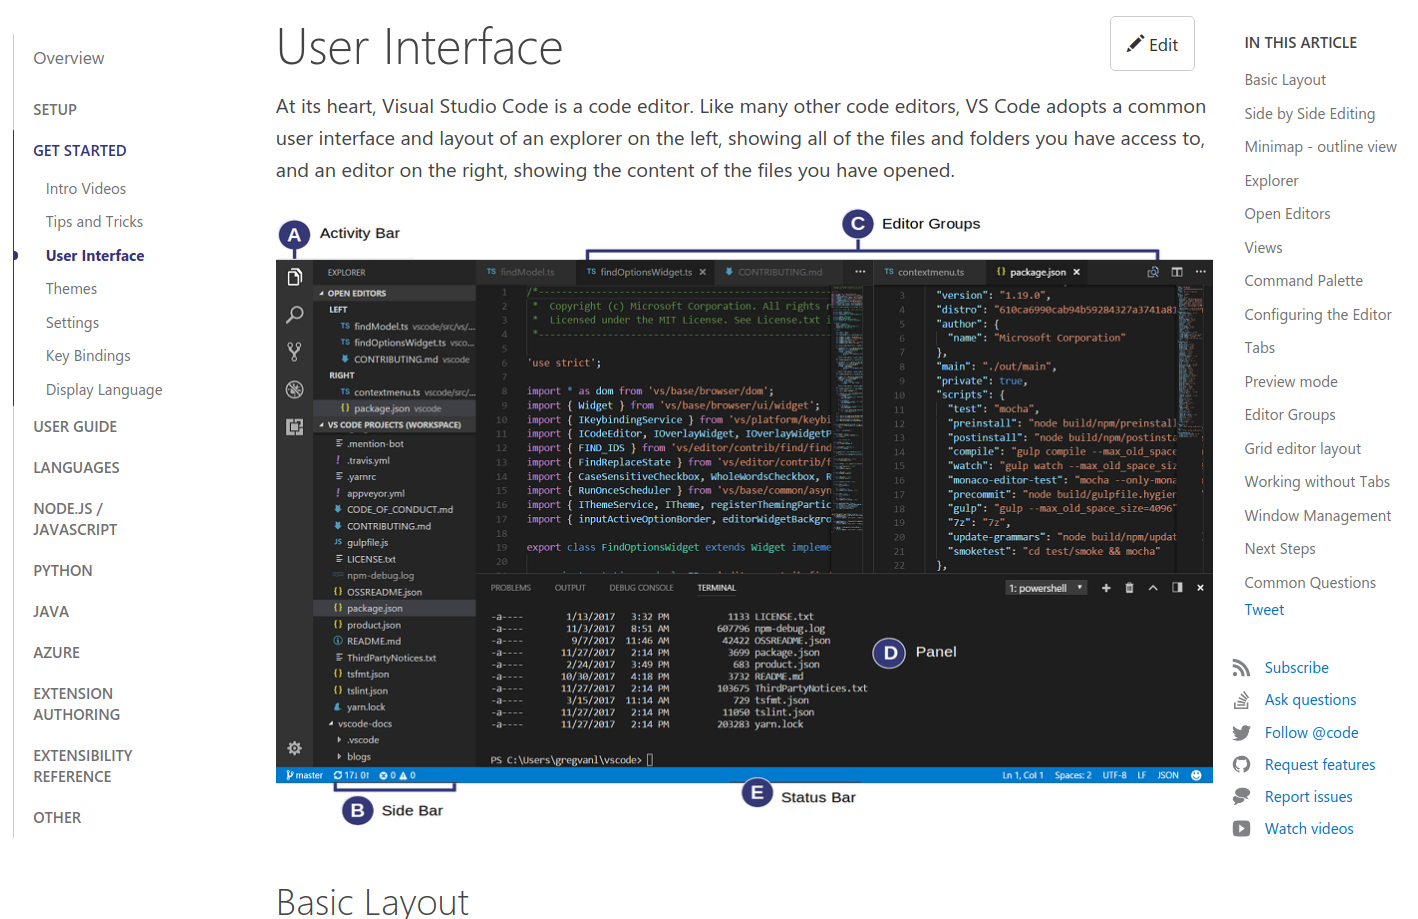
\includegraphics[width=0.9\textwidth]{imgs/VisualCode.png}
% 	\end{center}

% 	\href{https://code.visualstudio.com/}{Home page del tool: \url{https://code.visualstudio.com/}}

% \end{frame}


% %frame 0
% \begin{frame}
% 	\frametitle{Validatore XML}
% 	\framesubtitle{XMLlint}
% 	\addtocounter{nframe}{1}

% 	\begin{center}
% 		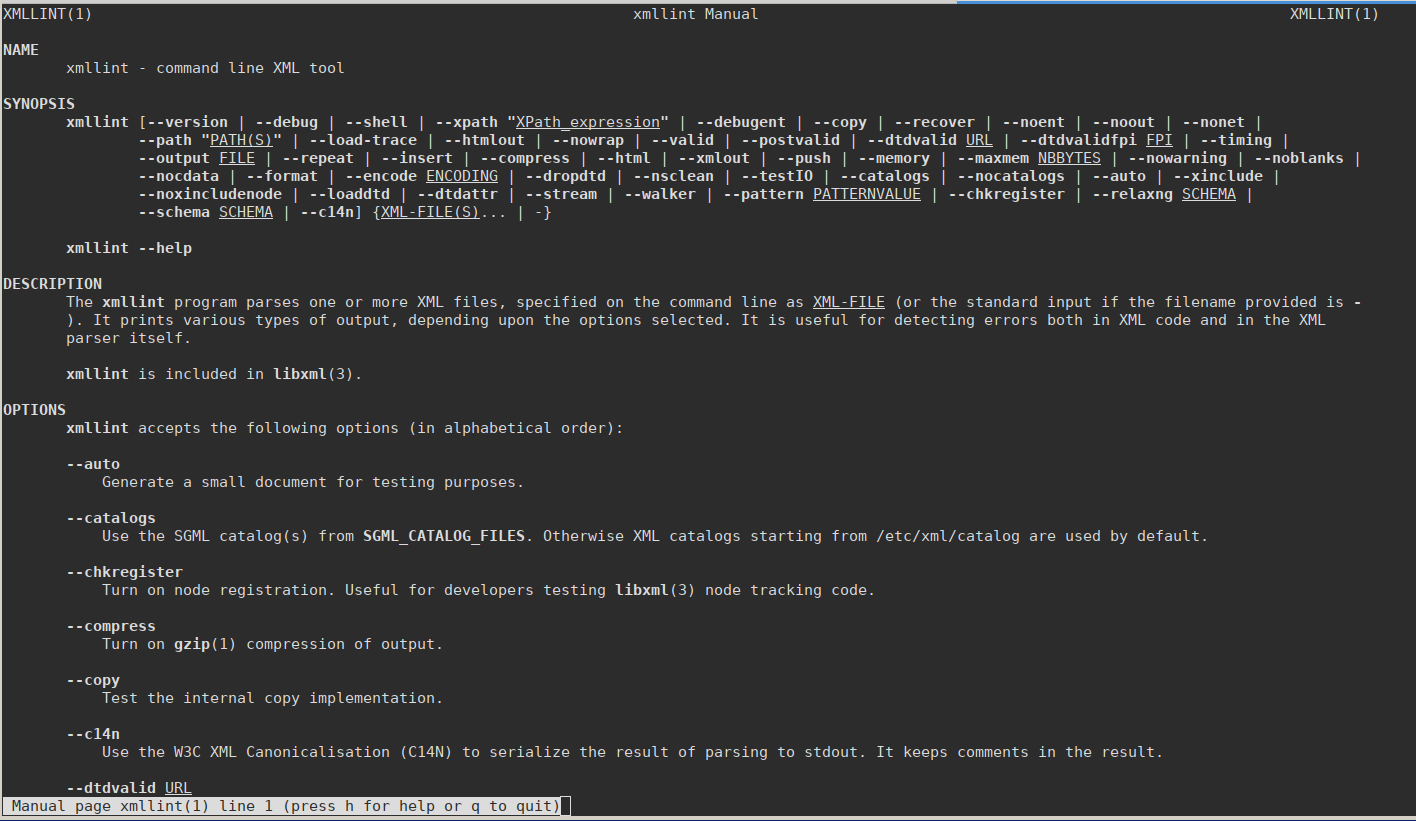
\includegraphics[width=0.9\textwidth]{imgs/XMLLINT.png}
% 	\end{center}

% 	\href{http://www.xmlsoft.org/}{Home page del tool: \url{http://www.xmlsoft.org/}}


% \end{frame}

% % frame 0
% \begin{frame}
% 	\frametitle{Editor XML}
% 	\framesubtitle{Cosa è consigliato usare}
% 	\addtocounter{nframe}{1}

% 	\begin{itemize}
% 		\item un buon editor open source: XML Copy Editor (http://xmlcopy-editor.sourceforge.net/)
% 		\item per Mac: XMLSpear, Textmate, Eclipse, IntelliJIDEA
% 		\item un ottimo editor: Oxygen (http://www.oxygenxml.com/) - multi piattaforma, ma non gratuito (in prova gratuita per un mese)
% 		\item altri editor: funzioni fondamentali sono la validazione, l’autocompletamento, l’esecuzione di fogli di stile
% 	\end{itemize}

% \end{frame}

% \begin{frame}
% 	\frametitle{Editor XML}
% 	\framesubtitle{EditiX}
% 	\addtocounter{nframe}{1}

% 	\begin{center}
% 		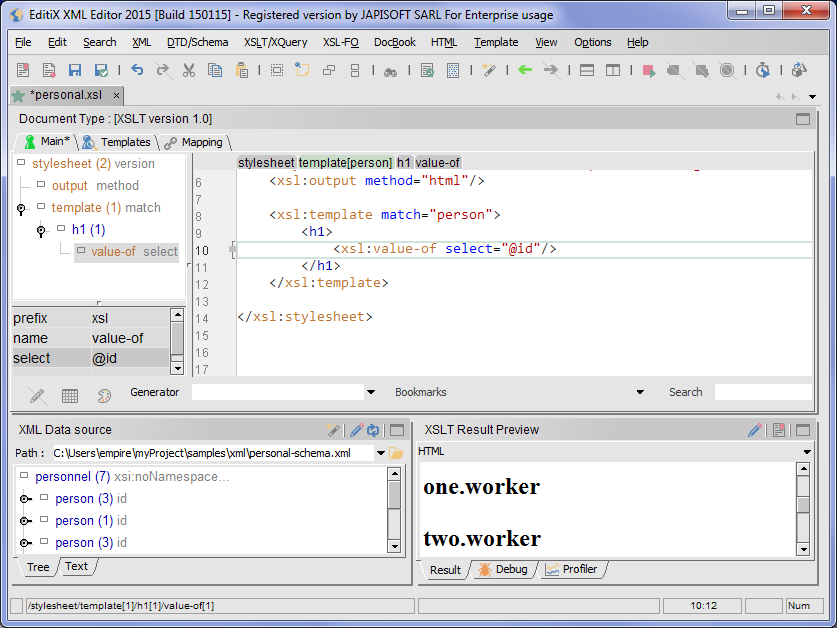
\includegraphics[width=0.8\textwidth]{imgs/maxi2.png}
% 	\end{center}

% 	\href{http://www.editix.com}{Home page del tool: \url{http://www.editix.com}}


% \end{frame}

% % frame 0
% \begin{frame}
% 	\frametitle{Programma d’esame}
% 	\framesubtitle{Cosa bisogna fare per superare l'esame}
% 	\addtocounter{nframe}{1}

% 	\begin{itemize}
% 		\item Studiare i lucidi delle lezioni
% 		\item Padroneggiare gli esercizi svolti durante il corso
% 		\item Studiare i testi indicati dal docente
% 		\item Studiare i capitoli delle Guidelines TEI che riguardano il corso e il progetto
% 		\item Realizzare il progetto di codifica concordato con il docente
% 	\end{itemize}

% \end{frame}

% % frame 0
% \begin{frame}
% 	\frametitle{Modalità d’esame}
% 	\framesubtitle{In cosa consiste l'esame}
% 	\addtocounter{nframe}{1}

% 	\begin{itemize}
% 		\item Invio del progetto (obbligatoriamente tramite github)
% 		\item Colloquio
% 		      \begin{itemize}
% 			      \item Discussione del progetto
% 			      \item Verifica delle conoscenze di base XML, XSD, XSL
% 			      \item Verifica delle basi teoriche
% 			      \item Conoscenza di TEI P5 (moduli principali, parti spiegate a lezione, moduli particolari utilizzati nel progetto)
% 		      \end{itemize}
% 	\end{itemize}

% \end{frame}

% % sezione Conclusioni frame 0
% \begin{frame}
% 	\frametitle{Materiale didattico}
% 	\framesubtitle{Riferimenti per studiare}
% 	\addtocounter{nframe}{1}

% 	\begin{block}{Slide}
% 		\begin{itemize}
% 			\item Slide delle lezioni corso a.a. 2018-2019
% 			\item Materiale integrativo fornito dal docente
% 			\item Repo github del corso \href{https://github.com/angelodel80/corsoCodifica}{\url{https://github.com/angelodel80/corsoCodifica}}
% 		\end{itemize}
% 	\end{block}


% \end{frame}

% \begin{frame}
% 	\frametitle{Materiale didattico}
% 	\framesubtitle{Riferimenti per studiare}
% 	\addtocounter{nframe}{1}

% 	\begin{block}{Libri}
% 		\begin{itemize}
% 			\item Burnard, L. (2014). What is the Text Encoding Initiative? How to add intelligent markup to digital resources. Marseille: OpenEdition Press.
% 			\item Ciotti, F. (2007). Il testo e l’automa: saggi di teoria e critica computazionale dei testi letterari. Aracne.
% 			\item Goldberg, K. H. (2010). XML: Visual QuickStart Guide. Pearson Education.
% 			\item Carey, P., and Vodnik, S. (2014). New Perspectives on XML, Comprehensive. Cengage Learning.			
% 		\end{itemize}

% 	\end{block}
% \end{frame}

% \begin{frame}
% 	\frametitle{Materiale didattico}
% 	\framesubtitle{Riferimenti per studiare}
% 	\addtocounter{nframe}{1}

% 	\begin{block}{Siti Web}
% 		\begin{itemize}
% 			\item \href{https://www.w3.org/XML/}{\url{http://www.tei-c.org/}}
% 			\item \href{http://teibyexample.org/}{\url{http://teibyexample.org/}}
% 			\item \href{https://www.w3.org/standards/xml/}{\url{https://www.w3.org/standards/xml/}}
% 		\end{itemize}

% 	\end{block}

% \end{frame}




\section{References}
% bibliografia di riferimento
%% Ciotti
%% Burnard
%% TEI guide lines
%% Pierazzo (due libri)
%% Slide (del corso)
%% XML specification e technical report W3C (https://www.w3.org/TR/xml/)
%% XML visual
%% XSL XPATH
%% XSD (art of XSD - SQL validation)
%% DTD (libro visual XML)
%% RELAXNG (libro relaxng, tutorial)

%bibliografia
\begin{frame}
    \frametitle{References}
    \addtocounter{nframe}{1}
    \begin{thebibliography}{10}
        \setbeamertemplate{bibliography item}[paper]
        \tiny\bibitem{Lenci2016} Lenci, A., Montemagni S., and Pirrelli V. (2016). Testo e Computer. Elementi Di Linguistica Computazionale. Aulamagna. Carocci.
        \tiny\bibitem{Pierazzo2015} Pierazzo, E. (2015). Digital Scholarly Editing : Theories, Models and Methods. Farnham Surrey: Ashgate.
        \tiny\bibitem{orlandi2010} Orlandi, T. (2010). Informatica testuale: teoria e prassi. Laterza.
        \tiny\bibitem{Pierazzo2016} Driscoll, M. J., and Pierazzo, E. (Eds.). (2016). Digital Scholarly Editing: Theories and Practices (Vol. 4). Open Book Publishers.
        \tiny\bibitem{ciotti2012} Ciotti F., e Crupi G, a c. di. (2012). Dall’Informatica umanistica alle culture digitali. ROMA : Casa Editrice Università La Sapienza. \href{http://www.editricesapienza.it/node/7688}{open access: http://www.editricesapienza.it/node/7688}
        \tiny\bibitem{Williams2009} Williams, I. (2009). Beginning XSLT and XPath: Transforming XML Documents and Data. Wiley.
        \tiny\bibitem{Kay2011} Kay, M. (2011). XSLT 2.0 and XPath 2.0 Programmer’s Reference. Wiley.
    \end{thebibliography}

\end{frame}

\begin{frame}
    \frametitle{References}
    \addtocounter{nframe}{1}
    \begin{thebibliography}{10}
        
        \setbeamertemplate{bibliography item}[online]
        \tiny\bibitem{MSDN} \textit{XML Standards Reference}, MSDN. \url{https://msdn.microsoft.com/en-us/library/ms256177(v=vs.110).aspx}
        \tiny\bibitem{IBMXML1} IBM XML \textit{Tutorial}, \url{https://www.ibm.com/developerworks/xml/tutorials/xmlintro/xmlintro.html}
        \tiny\bibitem{w3school} W3School Tutorial \url{https://www.w3schools.com/xml/default.asp}

    \end{thebibliography}

\end{frame}


\end{document}